% abtex2-modelo-trabalho-academico.tex, v-1.9.7 laurocesar
% Modelo de Trabalho Acadêmico (tese de doutorado, dissertação de
% mestrado e trabalhos monográficos em geral) em conformidade com 
% ABNT NBR 14724:2011
% ------------------------------------------------------------------------

\documentclass[
	% -- opções da classe memoir --
	12pt,				% tamanho da fonte
	%openright,			% seções começam em pág ímpar (insere página vazia caso preciso)
	oneside,			% para impressão em verso e anverso. Oposto a oneside
	a4paper,			% tamanho do papel. 
	% -- opções da classe abntex2 --
	%chapter=TITLE,		% títulos de seções principais convertidos em letras maiúsculas
	%section=TITLE,		% títulos de seções convertidos em letras maiúsculas
	%subsection=TITLE,	% títulos de subseções convertidos em letras maiúsculas
	%subsubsection=TITLE,% títulos de subsubseções convertidos em letras maiúsculas
	% -- opções do pacote babel --
	english,			% idioma adicional para hifenização
	french,				% idioma adicional para hifenização
	spanish,			% idioma adicional para hifenização
	brazil				% o último idioma é o principal do documento
	]{abntex2}

% ---
% PACOTES
% ---

% Pacotes básicos 
\usepackage{lmodern}			% Usa a fonte Latin Modern			
\usepackage[T1]{fontenc}		% Selecao de codigos de fonte.
\usepackage[utf8]{inputenc}		% Codificacao do documento (conversão automática dos acentos)
\usepackage{indentfirst}		% Indenta o primeiro parágrafo de cada seção.
\usepackage{textcomp}			% Símbolos adicionais
\usepackage{color}				% Controle das cores
\usepackage{graphicx}			% Inclusão de gráficos
\usepackage{microtype} 			% para melhorias de justificação
\usepackage{amsmath}
\usepackage{amssymb}
\usepackage{mathtools}
\usepackage{longtable}
\usepackage{booktabs}
\usepackage{multirow}           % Para células multi-linha em tabelas
\usepackage{csquotes}           % Para aspas corretas
\usepackage{float}              % Para forçar posicionamento de figuras com [H]
\usepackage{placeins}           % Para controlar onde floats podem ir com \FloatBarrier

% Configuração para melhorar posicionamento de figuras
\renewcommand{\topfraction}{0.85}        % máximo da página que pode ser ocupado por floats no topo
\renewcommand{\bottomfraction}{0.7}     % máximo da página que pode ser ocupado por floats no fundo
\renewcommand{\textfraction}{0.15}      % mínimo da página que deve ser texto
\renewcommand{\floatpagefraction}{0.66} % mínimo da página de floats que deve estar ocupada
\setcounter{topnumber}{3}
\setcounter{bottomnumber}{3}
\setcounter{totalnumber}{4}

% Pacotes de citações
\usepackage[brazilian,hyperpageref]{backref}	 % Paginas com as citações na bibl
\usepackage[alf,abnt-url=yes,abnt-emphasize=bf]{abntex2cite}	% Citações padrão ABNT

% Configuração para quebra de URLs longas
\PassOptionsToPackage{hyphens}{url}

% --- 
% CONFIGURAÇÕES DE PACOTES
% --- 

% Configurações do pacote backref
\renewcommand{\backrefpagesname}{Citado na(s) página(s):~}
% Texto padrão antes do número das páginas
\renewcommand{\backref}{}
% Define os textos da citação
\renewcommand*{\backrefalt}[4]{
	\ifcase #1 %
		Nenhuma citação no texto.%
	\or
		Citado na página #2.%
	\else
		Citado #1 vezes nas páginas #2.%
	\fi}%
% ---

% ---
% Informações de dados para CAPA e FOLHA DE ROSTO
% ---
\titulo{IMPACTO DE ESTAÇÕES METEOROLÓGICAS NA PRODUTIVIDADE AGRÍCOLA: UMA APLICAÇÃO DE DIFERENÇAS EM DIFERENÇAS COM TRATAMENTO ESCALONADO}
\autor{Daniel Cavalli}
\local{Rio de Janeiro}
\data{Dezembro 2025}
\orientador{Prof. Romero Rocha}
\instituicao{%
  UNIVERSIDADE FEDERAL DO RIO DE JANEIRO
  \par
  INSTITUTO DE ECONOMIA
  \par
  CURSO DE GRADUAÇÃO EM CIÊNCIAS ECONÔMICAS}
\tipotrabalho{Monografia}
% Preâmbulo: tipo do trabalho, objetivo, instituição e área de concentração 
\preambulo{Monografia apresentada ao Instituto de Economia da Universidade Federal do Rio de Janeiro como parte dos requisitos necessários à obtenção do título de Bacharel em Ciências Econômicas.}
% ---

% ---
% Configurações de aparência do PDF final

% alterando o aspecto da cor azul
\definecolor{blue}{RGB}{41,5,195}

% informações do PDF
\makeatletter
\hypersetup{
     	breaklinks=true,			% permite quebra de links em múltiplas linhas
     	%pagebackref=true,
		pdftitle={\@title}, 
		pdfauthor={\@author},
    	pdfsubject={\imprimirpreambulo},
	    pdfcreator={LaTeX with abnTeX2},
		pdfkeywords={estações meteorológicas}{PIB agropecuário}{diferenças em diferenças escalonada}{Callaway e Sant'Anna}{informação climática}, 
		colorlinks=true,       		% false: boxed links; true: colored links
    	linkcolor=blue,          	% color of internal links
    	citecolor=blue,        		% color of links to bibliography
    	filecolor=magenta,      	% color of file links
		urlcolor=blue,
		bookmarksdepth=4
}
\makeatother
% --- 

% --- 
% Espaçamentos entre linhas e parágrafos 
% --- 

% O tamanho do parágrafo é dado por:
\setlength{\parindent}{1.3cm}

% Controle do espaçamento entre um parágrafo e outro:
\setlength{\parskip}{0.2cm}  % tente também \onelineskip

% ---
% compila o indice
% ---
\makeindex
% ---

% ---
% Inclui valores gerados automaticamente
% Arquivo gerado automaticamente por generate_latex_values.r
% Última atualização: 2025-09-07

% Valores do teste placebo aleatório
\newcommand{\placebotruatt}{0.082}
\newcommand{\placebopvalue}{< 0,001}
\newcommand{\placebolower}{-0.037}
\newcommand{\placeboupper}{0.033}
\newcommand{\placebonsims}{50}
\newcommand{\placebomean}{-0.002}

% Valores formatados para texto
\newcommand{\placebotruattpct}{8.2\%}
\newcommand{\placebopvaluepct}{< 1\%}

% Valores do modelo principal
\newcommand{\mainatt}{0.082}
\newcommand{\mainse}{0.032}
\newcommand{\mainattpct}{8.2\%}

% Valores da análise de sensibilidade temporal
% Completo (2003-2023)
\newcommand{\sensfullatt}{0.126}
\newcommand{\sensfullse}{0.029}
\newcommand{\sensfulllower}{0.070}
\newcommand{\sensfullupper}{0.182}
\newcommand{\sensfulln}{7371}
% Excluindo Início (2006-2023)
\newcommand{\sensnostartatt}{0.130}
\newcommand{\sensnostartse}{0.031}
\newcommand{\sensnostartlower}{0.069}
\newcommand{\sensnostartupper}{0.191}
\newcommand{\sensnostartn}{6318}
% Excluindo Final (2003-2019)
\newcommand{\sensnoendatt}{0.117}
\newcommand{\sensnoendse}{0.027}
\newcommand{\sensnoendlower}{0.065}
\newcommand{\sensnoendupper}{0.170}
\newcommand{\sensnoendn}{5967}
% Excluindo COVID (2003-2019)
\newcommand{\sensnocovidatt}{0.117}
\newcommand{\sensnocovidse}{0.026}
\newcommand{\sensnocovidlower}{0.066}
\newcommand{\sensnocovidupper}{0.169}
\newcommand{\sensnocovidn}{5967}
% Pré-COVID (2003-2019)
\newcommand{\sensprecovidatt}{0.117}
\newcommand{\sensprecovidse}{0.025}
\newcommand{\sensprecovidlower}{0.068}
\newcommand{\sensprecovidupper}{0.167}
\newcommand{\sensprecovidn}{5967}

% ---

% ---
% Configuração para seções com quebra de página
% ---
\makeatletter
% Mantém quebra de página entre as seções principais
% \renewcommand{\clearforchapter}{}  % Comentado para manter quebras de página
\makeatother

% ---
% Configuração de espaçamentos das seções conforme ABNT
% ---
% ABNT: 2 espaços de 1,5 entrelinhas antes do título
\setlength{\beforechapskip}{3\baselineskip}
% ABNT: 1 espaço de 1,5 entrelinhas depois do título
\setlength{\afterchapskip}{1.5\baselineskip}

% Ajusta também o espaçamento das seções
\setlength{\beforesecskip}{1.5\baselineskip}
\setlength{\aftersecskip}{1.5\baselineskip}
% ---

% ----
% Início do documento
% ----
\begin{document}

% Idioma principal do documento
\selectlanguage{brazil}

% Remove espaços extras entre frases
\frenchspacing 

% ----------------------------------------------------------
% ELEMENTOS PRÉ-TEXTUAIS
% ----------------------------------------------------------
% \pretextual

% ---
% Capa
% ---
\imprimircapa
% ---

% ---
% Folha de rosto
% (o * indica que haverá a ficha bibliográfica)
% ---
\imprimirfolhaderosto*
% ---

% ---
% Inserir folha de aprovação
% ---

% Folha de aprovação - elemento obrigatório da NBR 14724/2011 (seção 4.2.1.3)
% Após a defesa, incluir a versão assinada pela banca:
% \includepdf{folhadeaprovacao_final.pdf}
\begin{folhadeaprovacao}

  \begin{center}
    {\ABNTEXchapterfont\large\imprimirautor}

    \vspace*{\fill}\vspace*{\fill}
    \begin{center}
      \ABNTEXchapterfont\bfseries\Large\imprimirtitulo
    \end{center}
    \vspace*{\fill}
    
    \hspace{.45\textwidth}
    \begin{minipage}{.5\textwidth}
        \imprimirpreambulo
    \end{minipage}%
    \vspace*{\fill}
   \end{center}
        
   Trabalho aprovado. \imprimirlocal, \today:

   \assinatura{\textbf{\imprimirorientador} \\ Orientador} 
   \assinatura{\textbf{Professor} \\ Convidado 1}
   \assinatura{\textbf{Professor} \\ Convidado 2}
      
   \begin{center}
    \vspace*{0.5cm}
    {\large\imprimirlocal}
    \par
    {\large\imprimirdata}
    \vspace*{1cm}
  \end{center}
  
\end{folhadeaprovacao}
% ---

% ---
% Agradecimentos
% ---
\begin{agradecimentos}

Agradeço à minha família, que sempre me apoiou durante toda a graduação sem nunca me pressionar além do necessário. Vocês foram fundamentais para que eu pudesse acumular o conhecimento necessário para montar este trabalho.

À minha namorada, Juliana, obrigado por me incentivar a terminar a faculdade e o TCC quando eu já não tinha mais vontade ou razão para tal. Seu apoio fez toda a diferença em me convencer da importância disso.

À minha cachorra, Moana, companheira fiel de tantas horas de escrita, modelagem e análise de dados. Sua presença tornou as longas madrugadas de trabalho muito mais suportáveis.

À Cláudia.

\end{agradecimentos}
% ---

% ---
% Epígrafe
% ---
\begin{epigrafe}
    \vspace*{\fill}
	\begin{flushright}
		\textit{``In mathematics you don't understand things.\\
		You just get used to them.''}\\
		(John von Neumann)
	\end{flushright}
\end{epigrafe}
% ---

% ---
% RESUMOS
% ---

% resumo em português
\setlength{\absparsep}{18pt} % ajusta o espaçamento dos parágrafos do resumo
\begin{resumo}
Este estudo examina o impacto causal da instalação de estações meteorológicas automáticas sobre o Produto Interno Bruto (PIB) agropecuário no Brasil, utilizando dados em painel de 490 microrregiões produtoras de cana-de-açúcar entre 2003 e 2023. Empregamos o arcabouço de Diferenças em Diferenças com adoção escalonada proposto por Callaway e Sant'Anna (2021), demonstrando sua aplicação em contextos de tratamento escalonado. A estratégia de identificação explora a variação temporal e geográfica na instalação de estações entre microrregiões eventualmente tratadas, utilizando o método "not-yet-treated" como grupo de controle dinâmico. Os resultados principais, obtidos através do estimador doubly robust, indicam um Efeito Médio do Tratamento sobre os Tratados (ATT) de \mainattpct{} (IC 95\%: [1,9\%; 14,5\%], p = 0,0103), representando ganhos econômicos significativos no setor agropecuário. A análise de event study revela ausência de tendências pré-tratamento diferenciadas, validando a estratégia de identificação. Testes extensivos de robustez confirmam a validade causal: placebos com PIB não-agropecuário (ATT não significativo), randomização múltipla (p-valor empírico < 0,01), múltiplas especificações alternativas (IPW: 9,4\%, REG: 6,6\%), e estabilidade temporal. Além dos resultados substantivos sobre produtividade agrícola, este trabalho serve como um guia prático para aplicação do arcabouço de Callaway e Sant'Anna no contexto de avaliação de políticas públicas com múltiplos períodos de tratamento. A disponibilização completa do código e documentação reforça o compromisso com transparência e reprodutibilidade na pesquisa econométrica aplicada.

 \textbf{Palavras-chave}: estações meteorológicas. produtividade agrícola. PIB agropecuário. diferenças em diferenças escalonada. Callaway e Sant'Anna. informação climática. avaliação de políticas públicas.
\end{resumo}

% resumo em inglês
\begin{resumo}[Abstract]
 \begin{otherlanguage*}{english}
This study examines the causal impact of automatic weather station installation on agricultural GDP in Brazil, using panel data from 490 sugarcane-producing microregions between 2003 and 2023. We employ the staggered adoption Differences-in-Differences framework proposed by Callaway and Sant'Anna (2021), demonstrating its superiority over traditional methods in contexts with multiple treatment periods. The identification strategy exploits temporal and geographic variation in station installation among eventually treated microregions, using the "not-yet-treated" method as a dynamic control group. The main results, obtained through the doubly robust estimator, indicate an average treatment effect (ATT) of 8.2\% (95\% CI: [1.9\%; 14.5\%], p = 0.0103), representing economically significant gains in agricultural GDP. The event study analysis reveals absence of differential pre-treatment trends, validating the identification strategy. Extensive robustness tests confirm causal validity: non-agricultural GDP placebos (non-significant ATT), multiple randomization (empirical p-value < 0.01), alternative specifications (IPW: 9.4\%, REG: 6.6\%), and temporal stability analysis. Beyond substantive findings on agricultural productivity, this work serves as a practical guide for applying the Callaway and Sant'Anna framework in the context of public policy evaluation with multiple treatment periods. Complete code and documentation availability reinforces commitment to transparency and reproducibility in applied econometric research.

   \textbf{Keywords}: weather stations. agricultural productivity. agricultural GDP. staggered differences-in-differences. Callaway and Sant'Anna. climate information. policy evaluation. Brazil.
 \end{otherlanguage*}
\end{resumo}

% ---
% inserir lista de ilustrações
% ---
\pdfbookmark[0]{\listfigurename}{lof}
\listoffigures*
\cleardoublepage
% ---

% ---
% inserir lista de tabelas
% ---
\pdfbookmark[0]{\listtablename}{lot}
\listoftables*
\cleardoublepage
% ---

% ---
% inserir o sumario
% ---
\pdfbookmark[0]{\contentsname}{toc}
\tableofcontents*
\cleardoublepage
% ---

% ----------------------------------------------------------
% ELEMENTOS TEXTUAIS
% ----------------------------------------------------------
\textual

% ----------------------------------------------------------
% INTRODUÇÃO INTEGRADA - VERSÃO UNIFICADA
% ----------------------------------------------------------
\chapter{Introdução}
\label{cap:introducao}

% Abertura forte conectando o problema econômico central
A agricultura brasileira enfrenta o desafio permanente de aumentar a produtividade em um contexto de crescente variabilidade climática. Com a produção agrícola global sendo amplamente determinada por oscilações meteorológicas durante o ciclo produtivo \cite{monteiro2009}, e as mudanças climáticas já impactando significativamente a produtividade mundial \cite{ortiz2020}, a questão central não é mais \textit{se} o clima afeta a agricultura, mas \textit{como} mitigar seus efeitos adversos e aproveitar janelas de oportunidade. Neste contexto, a informação meteorológica precisa emerge como insumo produtivo crítico, potencialmente capaz de transformar incerteza em risco gerenciável.

% Desenvolvimento do argumento com suporte da literatura
A literatura documenta extensivamente os canais através dos quais informações meteorológicas podem aumentar a produtividade agrícola. \citeonline{mavi2004} identificam três dimensões principais: planejamento estratégico (escolha de culturas e épocas de plantio), decisões táticas (timing de irrigação, aplicação de defensivos) e construção de resiliência sistêmica. \citeonline{weiss2000} demonstram que estações meteorológicas locais permitem ajustes finos nas práticas agrícolas, enquanto \citeonline{rijks2000} quantificam os ganhos econômicos potenciais de serviços meteorológicos bem estruturados. No Brasil, sistemas como AGRITEMPO e SISDAGRO já operacionalizam essas informações, mas sua efetividade depende crucialmente da densidade e qualidade da rede de estações meteorológicas subjacente.

% Mecanismo causal explícito
O mecanismo causal pode ser descrito de forma sequencial: a instalação de uma estação meteorológica local gera dados climáticos precisos e em tempo real, que são processados e disponibilizados aos produtores através de boletins, alertas e sistemas de informação. Com acesso a previsões mais acuradas sobre temperatura, precipitação e eventos extremos, os agricultores podem otimizar decisões críticas – desde o momento ideal de plantio e colheita até a aplicação precisa de insumos e gestão eficiente de irrigação. 

Além do uso direto pelos produtores, esses dados alimentam modelos computacionais avançados de simulação agrícola. Por exemplo, o modelo DSSAT CSM-CANEGRO, amplamente utilizado no setor sucroalcooleiro, integra informações meteorológicas locais para simular o crescimento e desenvolvimento da cana-de-açúcar sob diferentes cenários de manejo. Com dados meteorológicos precisos, o modelo permite aos agricultores testar virtualmente diferentes estratégias de irrigação, identificando configurações ótimas que podem resultar em incrementos de produtividade de até 30\%, especialmente em solos mais vulneráveis ao déficit hídrico \cite{vianna2016}. Essa capacidade de simular e otimizar decisões antes da implementação no campo representa um salto qualitativo na gestão agrícola.

Essas decisões melhor informadas – seja através do uso direto das previsões ou através de modelos de simulação alimentados por dados locais – traduzem-se em redução de perdas, aumento de produtividade e, consequentemente, crescimento do PIB agropecuário local.

% Identificação da lacuna crítica
Apesar do consenso teórico sobre a importância da informação meteorológica, existe uma lacuna crítica na literatura: \textbf{a ausência de evidências causais robustas sobre o impacto econômico da expansão da infraestrutura de monitoramento climático}. Estudos existentes são predominantemente descritivos ou baseados em correlações, deixando em aberto questões fundamentais: Qual é o retorno econômico da instalação de estações meteorológicas? Como esse impacto evolui ao longo do tempo? Os benefícios justificam os custos de expansão da rede?

% Desafio metodológico
A dificuldade em responder essas questões não é trivial. A instalação de estações meteorológicas no Brasil ocorreu de forma escalonada ao longo de duas décadas, com diferentes regiões adotando a tecnologia em momentos distintos. Este padrão de "adoção escalonada" (staggered adoption) invalida o uso de métodos econométricos tradicionais. Como demonstrado por \citeonline{goodman2021} e \citeonline{sun2021}, o estimador de Diferenças em Diferenças com Efeitos Fixos Bidimensionais (Two-Way Fixed Effects - TWFE) – padrão ouro em avaliações de impacto – produz resultados enviesados neste contexto, pois inadvertidamente usa unidades já tratadas como controles e confunde efeitos heterogêneos ao longo do tempo.

% Proposta e contribuição principal
Este trabalho preenche essa lacuna ao estimar o \textbf{efeito causal da instalação de estações meteorológicas sobre o PIB agropecuário}, utilizando o arcabouço metodológico de \citeonline{callaway2021} para Diferenças em Diferenças com múltiplos períodos. É importante esclarecer que, embora utilizemos a produção de cana-de-açúcar como critério de seleção das microrregiões – dada sua relevância econômica e alta sensibilidade climática – nossa variável de resultado é o PIB agropecuário total, capturando assim os efeitos agregados sobre toda a produção agrícola local. 

Nossa análise revela que a instalação de estações meteorológicas gera um aumento de \textbf{\mainattpct{} no PIB agropecuário} das microrregiões tratadas. Estes resultados são robustos a múltiplas especificações, testes placebo e análises de sensibilidade, fornecendo evidência causal rigorosa sobre a efetividade desta política.

% Contribuições específicas
As contribuições deste trabalho são quádruplas:

\begin{enumerate}
\item \textbf{Evidência causal pioneira}: Primeira quantificação rigorosa do impacto econômico de estações meteorológicas na agricultura brasileira, preenchendo uma lacuna crítica para políticas públicas baseadas em evidências.

\item \textbf{Avanço metodológico}: Demonstração da aplicabilidade e importância dos novos métodos de DiD escalonado em contextos agrícolas, contribuindo para a literatura metodológica aplicada.

\item \textbf{Caracterização da dinâmica temporal}: Documentação do processo de difusão e aprendizado, com implicações para avaliação de investimentos em infraestrutura meteorológica.

\item \textbf{Subsídios para expansão da rede}: Evidências de que o retorno social supera amplamente os custos, justificando a expansão da infraestrutura meteorológica como estratégia de adaptação climática e aumento de produtividade.
\end{enumerate}

% Diálogo com literatura recente
Nossos resultados dialogam com desenvolvimentos recentes na literatura. \citeonline{burke2021} argumentam que avanços em tecnologias de informação representam uma das principais fronteiras para aumentar a produtividade agrícola no século XXI. \citeonline{monteiro2017} demonstram a importância de modelos agrometeorológicos para identificação de gaps de produtividade na agricultura brasileira. \citeonline{crost2018} e \citeonline{gatti2021} demonstram, usando métodos similares aos nossos, como infraestrutura pode mitigar impactos climáticos. Este trabalho contribui para essa literatura emergente ao fornecer a primeira evidência causal direta sobre estações meteorológicas.

% Estrutura do trabalho
O restante deste trabalho está organizado da seguinte forma. A Seção 2 apresenta a metodologia completa, incluindo o arcabouço de Diferenças em Diferenças com múltiplos períodos de \citeonline{callaway2021}, a estratégia empírica, definição do tratamento, variáveis e especificação do modelo. A Seção 3 apresenta os resultados, começando pela implementação computacional e seguindo com os efeitos estimados, análises de robustez e testes de validação. A Seção 4 conclui com implicações para políticas públicas e direções para pesquisa futura.

% ----------------------------------------------------------
% Metodologia
% ----------------------------------------------------------
\chapter{Metodologia}

Para este trabalho, utilizaremos como principal referência o artigo de \citeonline{callaway2021}, que apresenta uma extensão do modelo de Diferenças em Diferenças (DiD) para cenários com múltiplos períodos e momentos distintos de adoção do tratamento.

\section{Introdução ao Modelo}

No DiD clássico, assume-se um grupo tratado que recebe a intervenção em um momento específico e um grupo controle que nunca é tratado. Sob essa configuração, a diferença no tempo entre pré e pós-tratamento e a diferença entre grupos tratado e controle fornecem a estimativa do efeito causal. Entretanto, para o caso analisado neste trabalho há múltiplos períodos e vários grupos recebendo o tratamento em momentos distintos ao longo dos 22 anos do período de análise. A abordagem de DiD tradicional, nesse caso, pode gerar estimativas enviesadas devido à heterogeneidade do tratamento ao longo do tempo, resultando em interpretação ambígua.

O modelo de \citeonline{callaway2021} surge como uma forma de permitir que esses cenários de tratamento escalonado, frequentemente mais comuns no mundo real do que experimentos naturais, possam ser avaliados adequadamente. Por permitir a identificação de efeitos médios do tratamento específicos para cada grupo e período, acomoda a heterogeneidade do momento de adoção e suas dinâmicas, além de fornecer uma interpretação mais clara dos parâmetros causais.

\section{Fundamentos do modelo}

O modelo proposto pode ser entendido em três etapas conceituais:

\begin{enumerate}
\item \textbf{Identificação de parâmetros causais desagregados:} Primeiro, são obtidas estimativas do efeito causal para cada combinação de grupo tratado e período após a adoção (denotados por ATT(g,t)), focando em captar o efeito específico para um determinado conjunto de unidades tratadas em um dado momento do tempo.

\item \textbf{Agregação desses parâmetros:} Em seguida, esses parâmetros individuais, definidos para grupos e períodos específicos, podem ser combinados para produzir medidas resumidas de efeitos, como efeitos médios globais, ao longo do tempo, por coorte de tratamento ou segundo o tempo decorrido desde a intervenção.

\item \textbf{Estimação e inferência:} Por fim, procedimentos estatísticos são empregados para estimar esses parâmetros, bem como inferir sobre sua significância estatística.
\end{enumerate}

\subsection{Group-Time Average Treatment Effects ATT(g,t)}

O parâmetro fundamental dessa abordagem é o ATT(g,t), que representa o Efeito Médio do Tratamento para o grupo g no período t. Ao contrário do DiD tradicional, onde há um único efeito estimado, aqui obtemos uma coleção de efeitos, cada um refletindo o impacto do tratamento em um grupo que começou a ser tratado em um determinado momento e está sendo avaliado em um período específico após o início do tratamento.

Com isso é possível capturar heterogeneidades relacionadas:
\begin{itemize}
\item Ao grupo (unidades diferentes podem ter características e contextos distintos);
\item Ao momento de início do tratamento (tratamentos iniciados em diferentes épocas podem ter efeitos variados devido a condições econômicas, políticas ou sociais);
\item Ao tempo decorrido desde o tratamento (efeitos imediatos versus efeitos de longo prazo podem diferir).
\end{itemize}

\subsection{Identificação}

O artigo de \citeonline{callaway2021} apresenta uma série de pressupostos para identificação dos parâmetros causais. Boa parte delas não difere muito dos pressupostos do DiD tradicional. Abaixo destaco algumas importantes mudanças:

\begin{enumerate}
\item \textbf{Tendências Paralelas Condicionais:} A ideia central do DiD é que, na ausência de tratamento, as unidades tratadas seguiriam a mesma tendência de evolução dos resultados das unidades não tratadas. Existem diferenças conceituais entre o DiD tradicional e o DiD Staggered:
   \begin{itemize}
   \item \textbf{Pressuposto 4 - ``never-treated'':} Aqui, o grupo de comparação é formado por unidades que nunca recebem tratamento ao longo de todo o período observado. Pressupõe-se que, condicionalmente a covariáveis observáveis, esses ``never-treated'' representam a contrafactual apropriada para o que teria acontecido com os grupos tratados caso não tivessem sido tratados.
   \item \textbf{Pressuposto 5 - ``not-yet-treated'':} Nesse caso, o grupo de controle para um determinado período e grupo tratado é formado por unidades que ainda não foram tratadas até aquele momento, mas que virão a ser tratadas no futuro. Essa abordagem aproveita a natureza escalonada do tratamento para criar um grupo de comparação internamente consistente.
   \end{itemize}

\item \textbf{Pressuposto 3 - Antecipação Limitada do Tratamento:} Admite-se que as unidades não são afetadas pelo tratamento antes de sua efetiva implementação, ou que se conheçam efeitos de antecipação limitados e controláveis. Caso haja antecipação, o modelo permite incorporar essa informação, desde que os períodos de antecipação sejam conhecidos e adequadamente modelados.

\item \textbf{Sobreposição (Overlap):} É necessário que haja sobreposição entre as características das unidades tratadas e as unidades de controle, garantindo que as diferenças observadas possam ser atribuídas ao tratamento e não a dessemelhanças estruturais entre grupos.
\end{enumerate}

\subsubsection{Validade dos Pressupostos no Contexto de Estações Meteorológicas}

É importante verificar como estes pressupostos se aplicam ao nosso contexto específico:

\textbf{No Anticipation}: No caso de estações meteorológicas, este pressuposto é amplamente, mas não perfeitamente, satisfeito. Embora as informações meteorológicas localizadas e precisas só existam após a instalação física da estação, reconhecemos que produtores podem utilizar dados de estações vizinhas, com menor precisão. Se houver algum grau de antecipação, nosso estimador tende a ser conservador, subestimando o verdadeiro impacto da estação, pois parte do efeito seria capturado antes do período oficial de tratamento. Isso fortalece nossas conclusões: se encontramos efeitos significativos mesmo com possível antecipação, o impacto real tende a ser ainda maior.

\textbf{Tratamento Irreversível}: Uma vez instalada, assume-se que a estação permanece operacional. Nossa análise não considera casos de desativação de estações, tratando a adoção como permanente (staggered adoption).

\textbf{Tendências Paralelas Condicionais}: Este é o pressuposto mais crítico e testável. Nossa análise fornece forte evidência empírica através do teste formal (F = 1,136, p = 0,3215) e da inspeção visual dos períodos pré-tratamento no event study, onde os coeficientes oscilam aleatoriamente em torno de zero sem tendência sistemática.

\subsection{Estimação}

Para estimar o ATT(g,t), são propostas três abordagens principais:

\begin{enumerate}
\item \textbf{Regressão de Resultado (Outcome Regression - OR):} Modela-se diretamente o resultado nos grupos de controle, condicionando a covariáveis pré-tratamento. O efeito é então obtido comparando a predição contrafactual com o resultado efetivo observado nas unidades tratadas.

\item \textbf{Ponderação por Probabilidade Inversa (Inverse Probability Weighting - IPW):} Aqui, pondera-se cada unidade pela probabilidade condicional de tratamento. Ao ajustar esses pesos, obtém-se um contrafactual equilibrado, simulando um cenário onde o tratamento foi aplicado aleatoriamente.

\item \textbf{Duplamente Robusto (Doubly Robust - DR):} Combina OR e IPW, resultando em um estimador robusto a erros de especificação. Mesmo se um dos modelos (resultado ou probabilidade) estiver incorretamente especificado, a consistência pode ser mantida. Na prática, essa abordagem é frequentemente recomendada por oferecer maior segurança em cenários reais, onde a especificação perfeita do modelo é incerta.
\end{enumerate}

\subsection{Agregação de Efeitos}

Após estimar os ATT(g,t) para cada combinação grupo-tempo, \citeonline{callaway2021} propõem diferentes esquemas de agregação para obter medidas resumidas do efeito do tratamento. A escolha do esquema de agregação depende da questão de pesquisa específica.

\subsubsection{Agregação Simples com Pesos Positivos}

Uma primeira possibilidade seria simplesmente fazer a média de todos os ATT(g,t) identificados:

\begin{equation}
\theta^O_W = \frac{1}{\kappa} \sum_{g \in \mathcal{G}} \sum_{t=2}^{T} \mathbf{1}\{t \geq g\} \cdot ATT(g,t) \cdot P(G = g | G \leq T)
\end{equation}

onde $\kappa = \sum_{g \in \mathcal{G}} \sum_{t=2}^{T} \mathbf{1}\{t \geq g\} \cdot P(G = g | G \leq T)$ garante que os pesos somem um.

Embora $\theta^O_W$ evite os problemas de pesos negativos do TWFE tradicional, ele tem a desvantagem de sistematicamente atribuir mais peso a grupos que participam do tratamento por mais tempo.

\subsubsection{Efeito Médio do Tratamento sobre os Tratados (Recomendado)}

Para superar essa limitação, \citeonline{callaway2021} recomendam o seguinte parâmetro como medida geral do efeito médio de participar do tratamento:

\begin{equation}
\theta^O_{sel} = \sum_{g \in \mathcal{G}} \theta_{sel}(g) \cdot P(G = g | G \leq T)
\end{equation}

onde $\theta_{sel}(g)$ é o efeito médio de participar do tratamento para unidades no grupo $g$:

\begin{equation}
\theta_{sel}(g) = \frac{1}{T - g + 1} \sum_{t=g}^{T} ATT(g,t)
\end{equation}

Este parâmetro primeiro calcula o efeito médio para cada grupo (através de todos os períodos pós-tratamento) e então faz a média desses efeitos entre grupos. Assim, $\theta^O_{sel}$ representa o efeito médio de participar do tratamento experimentado por todas as unidades que alguma vez participaram do tratamento. Sua interpretação é análoga ao ATT no DiD canônico com dois períodos e dois grupos.

\subsubsection{Agregações para Event Studies}

Para análises de event study que examinam a dinâmica temporal dos efeitos, utilizamos a agregação balanceada, que evita problemas de mudanças na composição dos grupos ao longo do tempo relativo ao tratamento.

\section{Especificação do Modelo}

Nossa análise baseia-se em um painel de dados escalonado que pode ser formalmente descrito como $\mathcal{D} = \{(Y_{it}, W_{it}, X_{it})\}_{i=1,t=1}^{N,T}$, onde:

\begin{itemize}
\item $N$: número total de unidades (microrregiões) no painel.
\item $T$: número total de períodos de tempo (anos) no painel.
\item $i \in \{1, 2, \ldots, N\}$: índice que identifica a unidade (microrregião).
\item $t \in \{1, 2, \ldots, T\}$: índice que identifica o período de tempo (ano).
\item $Y_{it}$: logaritmo do PIB agropecuário da microrregião $i$ no ano $t$.
\item $W_{it}$: indicador binário de tratamento (1 se a microrregião $i$ possui estação meteorológica ativa no ano $t$, 0 caso contrário).
\item $X_{it}$: vetor de covariadas da microrregião $i$ no ano $t$.
\end{itemize}

A abordagem de \citeonline{callaway2021} permite estimar o Efeito Médio do Tratamento sobre os Tratados (ATT) específico para cada coorte $g$ (grupo de unidades tratadas no mesmo período) e tempo $t$, denotado por $ATT(g,t)$. Estes efeitos podem então ser agregados de diferentes formas para obter estimativas de interesse para políticas públicas.


\subsection{Definição do Tratamento e Unidades de Análise}

O tratamento é definido como a instalação de pelo menos uma estação meteorológica automática em funcionamento na microrregião. A escolha da microrregião como unidade de análise justifica-se por três razões principais:

\begin{enumerate}
\item \textbf{Escala geográfica apropriada}: As microrregiões representam agrupamentos de municípios com características agroclimáticas similares, permitindo capturar adequadamente a área de influência das informações meteorológicas.

\item \textbf{Estabilidade institucional}: Diferentemente dos municípios, que podem sofrer desmembramentos, as microrregiões mantêm fronteiras estáveis ao longo do período analisado.

\item \textbf{Poder estatístico}: A agregação em microrregiões produtoras de cana-de-açúcar (490 unidades no total, com 303 apresentando dados pré-tratamento válidos) oferece um equilíbrio entre granularidade espacial e tamanho amostral suficiente para identificação robusta dos efeitos.
\end{enumerate}

\subsection{Construção dos Grupos de Tratamento}

Seguindo a notação de \citeonline{callaway2021}, definimos $G_i$ como o ano em que a microrregião $i$ recebe sua primeira estação meteorológica. Para unidades nunca tratadas durante o período de análise, convencionamos $G_i = 0$. Esta codificação é essencial para a implementação computacional e permite a utilização dessas unidades como grupo de controle potencial.

A distribuição temporal da adoção revela padrões relevantes: observa-se uma concentração significativa de instalações em 2006-2008, coincidindo com programas federais de expansão da rede meteorológica, seguida por adoção mais esparsa nos anos subsequentes. Das 490 microrregiões analisadas, a maioria eventualmente recebeu estações ao longo do período de estudo.

\subsection{Variável Dependente e Transformações}

A variável dependente principal é o logaritmo natural do PIB agropecuário, definida como:

\begin{equation}
Y_{it} = \ln(1 + \text{PIB\_Agropecuário}_{it})
\end{equation}

onde $\text{PIB\_Agropecuário}_{it}$ representa o valor total da produção agropecuária para a microrregião $i$ no ano $t$. A transformação logarítmica oferece três vantagens metodológicas importantes:

\begin{enumerate}
\item \textbf{Interpretação econômica direta}: Os coeficientes estimados podem ser interpretados aproximadamente como variações percentuais na produtividade, facilitando a comunicação dos resultados.

\item \textbf{Redução de heterocedasticidade}: A transformação log suaviza a variância crescente tipicamente observada em dados de produtividade agrícola.

\item \textbf{Tratamento de zeros}: O uso de $\ln(1+x)$ evita problemas computacionais quando há observações com produtividade zero, mantendo essas observações na amostra.
\end{enumerate}

\subsection{Covariáveis e Especificação do Modelo}

A especificação do modelo inclui um conjunto de covariáveis socioeconômicas cuidadosamente selecionadas para controlar por fatores que podem influenciar tanto a probabilidade de receber uma estação meteorológica quanto o PIB agropecuário:

\begin{enumerate}
\item \textbf{Log da área plantada}: Controla pelo tamanho da atividade agrícola na microrregião, capturando economias de escala e intensidade produtiva.

\item \textbf{Log da população}: Proxy para desenvolvimento econômico local e demanda por produtos agrícolas.

\item \textbf{Log do PIB per capita}: Captura o nível de desenvolvimento econômico e capacidade de investimento local.

\item \textbf{Log da densidade de estações na UF}: Variável construída agregando o número de estações meteorológicas ao nível estadual, normalizada pela área. Esta variável é crucial para capturar potenciais efeitos de spillover regional, reconhecendo que informações meteorológicas podem fluir entre microrregiões vizinhas dentro do mesmo estado.
\end{enumerate}

A inclusão da densidade estadual de estações merece destaque especial. Esta variável permite um pseudo-mapeamento dos efeitos de transbordamento regional, considerando que:

\begin{itemize}
\item Informações meteorológicas têm natureza de bem público, podendo beneficiar áreas além da localização física da estação
\item A instalação de estações melhora a qualidade das previsões meteorológicas para toda a região, criando um efeito sistêmico que se propaga principalmente dentro dos limites estaduais
\item Produtores podem se beneficiar indiretamente da maior densidade de estações no estado através de previsões mais precisas e dados climáticos mais confiáveis
\end{itemize}

\subsection{O Estimador Duplamente Robusto}

Para a estimação dos efeitos causais, adotamos o estimador \textit{Duplamente Robusto} (DR) proposto por \citeonline{santanna2020}, que combina modelos de regressão para o resultado com ponderação por probabilidade inversa. Esta abordagem oferece propriedades estatísticas desejáveis:

\begin{itemize}
\item \textbf{Dupla proteção contra má especificação}: O estimador permanece consistente se pelo menos um dos dois modelos (resultado ou score de propensão) estiver corretamente especificado.

\item \textbf{Eficiência melhorada}: Sob especificação correta de ambos os modelos, o DR atinge a fronteira de eficiência semiparamétrica.

\item \textbf{Robustez a extremos}: A combinação de métodos mitiga problemas associados a pesos extremos no IPW puro.
\end{itemize}

\subsection{Escolha do Grupo de Controle}

Uma decisão metodológica importante na implementação do estimador de \citeonline{callaway2021} refere-se à escolha do grupo de controle. O pacote \texttt{did} oferece duas opções principais:

\begin{itemize}
\item \textbf{Not-yet-treated}: Utiliza como controle tanto unidades nunca tratadas quanto unidades ainda não tratadas no período $t$. Esta abordagem maximiza o tamanho da amostra de controle e é particularmente útil em contextos com poucos ou nenhum never-treated.

\item \textbf{Never-treated}: Restringe o grupo de controle apenas às unidades que nunca receberam tratamento durante todo o período amostral. Embora conceitualmente mais limpo, pode resultar em poder estatístico reduzido.
\end{itemize}

Para esta análise, adotamos como padrão o grupo \textbf{not-yet-treated} por três razões: (i) maximiza a eficiência estatística ao utilizar toda a informação disponível; (ii) é apropriado para nosso contexto onde a adoção ocorre gradualmente ao longo do tempo; e (iii) os resultados mostram-se robustos a ambas as especificações (diferença de apenas 2,5\%), validando esta escolha metodológica.

\section{Especificação da Análise de Estudo de Evento}

A análise de estudo de evento constitui o núcleo da estratégia empírica adotada, permitindo examinar como o efeito do tratamento evolui dinamicamente ao longo do tempo. Esta abordagem é particularmente adequada para o contexto analisado por três razões fundamentais:

\begin{enumerate}
\item \textbf{Teste de tendências paralelas}: Permite verificar visualmente e estatisticamente se os grupos tratados e controle seguiam trajetórias similares antes do tratamento, validando o pressuposto fundamental de identificação.

\item \textbf{Dinâmica de adoção tecnológica}: Captura o processo gradual de difusão e aprendizado associado ao uso de informações meteorológicas, reconhecendo que os benefícios podem não ser imediatos.

\item \textbf{Heterogeneidade temporal}: Acomoda a possibilidade de que os efeitos variem com o tempo de exposição ao tratamento, seja por acumulação de conhecimento ou mudanças nas práticas agrícolas.
\end{enumerate}

\subsection{Formalização da Análise de Estudo de Evento}

Definimos o tempo relativo ao tratamento como $e = t - g$, onde $g$ é o ano de instalação da primeira estação e $t$ é o período calendário. Assim, $e < 0$ representa períodos pré-tratamento, $e = 0$ marca o início do tratamento, e $e > 0$ captura períodos pós-tratamento.

A agregação dos efeitos ATT(g,t) em função do tempo relativo segue a especificação:

\begin{equation}
\theta_{es}^{bal}(e) = \sum_{g \in \mathcal{G}} \mathbf{1}\{g + e \leq T\} \cdot P(G = g | G + e \leq T) \cdot ATT(g, g+e)
\end{equation}

onde:
\begin{itemize}
\item $\theta_{es}^{bal}(e)$ representa o efeito médio do tratamento $e$ períodos após sua introdução
\item $\mathcal{G}$ é o conjunto de coortes de adoção (excluindo nunca tratados)
\item $P(G = g | G + e \leq T)$ são pesos que garantem que cada coorte contribua proporcionalmente ao número de unidades tratadas
\item $\mathbf{1}\{g + e \leq T\}$ assegura que incluímos apenas coortes observadas por pelo menos $e$ períodos pós-tratamento
\end{itemize}

Esta especificação garante comparabilidade entre períodos, ponderando adequadamente a contribuição de cada coorte conforme sua representatividade na amostra.

É importante notar que, conforme alertam \citeonline{callaway2021}, event studies longos podem sofrer de mudanças na composição dos grupos contribuindo para cada período relativo. Em nosso caso, com tratamento escalonado de 2000 a 2019, períodos relativos extremos ($e > 15$ ou $e < -15$) são estimados com base em poucas coortes, o que explica a maior variabilidade observada nesses períodos. A agregação balanceada $\theta_{es}^{bal}(e)$ mitiga este problema ao fixar o conjunto de grupos contribuintes.

% ----------------------------------------------------------
% Resultados
% ----------------------------------------------------------
\chapter{Resultados}

\section{Implementação Computacional}

\subsection{Software e Pacotes Utilizados}

A implementação empírica foi realizada utilizando o software R \cite{rcoreteam2024} em conjunto com o pacote \texttt{did} (versão 2.1.2), desenvolvido por \citeonline{callaway2021}. O uso deste pacote oficial garante conformidade estrita com os procedimentos propostos no artigo metodológico, implementando fielmente os estimadores e procedimentos de inferência. As principais funcionalidades utilizadas incluem:

\begin{itemize}
\item Cálculo dos ATT(g,t) com inferência via bootstrap
\item Agregações flexíveis (overall, dynamic, group, calendar)
\item Diagnósticos de balanço e testes de especificação
\item Tratamento adequado de dados desbalanceados
\end{itemize}

Complementarmente, utilizamos os pacotes \texttt{dplyr} para manipulação de dados, \texttt{ggplot2} para visualizações, e \texttt{purrr} para programação funcional, garantindo reprodutibilidade através do sistema \texttt{renv} de gerenciamento de dependências.

\subsection{Transparência e Reprodutibilidade}

Em alinhamento com as melhores práticas de ciência aberta e transparência acadêmica, todo o código desenvolvido para este trabalho está disponível publicamente no repositório GitHub \url{https://github.com/danielcavalli/tcc-ie-ufrj-2024}. O repositório contém:

\begin{itemize}
\item Scripts de extração e preparação de dados em Python
\item Código completo do modelo econométrico em R
\item Arquivos \LaTeX\ do documento final
\item Bibliografia e referências utilizadas
\item Histórico completo de versionamento do projeto
\end{itemize}

A extração inicial dos dados foi realizada utilizando Python em conjunto com o pacote \texttt{basedosdados} e a API do Google BigQuery, permitindo acesso eficiente aos microdados do IBGE e outras fontes oficiais. Esta abordagem garante:

\begin{itemize}
\item \textbf{Rastreabilidade}: Todo o processo de obtenção e transformação dos dados está documentado
\item \textbf{Reprodutibilidade}: Qualquer pesquisador pode recriar o dataset a partir das fontes originais
\item \textbf{Transparência}: O versionamento completo permite acompanhar a evolução da análise
\end{itemize}

\subsection{Estrutura dos Dados e Processo de Extração}

O conjunto de dados foi construído através de um processo sistemático de extração e agregação utilizando Python, o pacote \texttt{basedosdados} e a API do Google BigQuery. O notebook \texttt{analise\_did\_microrregions.ipynb}, disponível no repositório do projeto, documenta todo o processo de construção do dataset. As etapas principais incluem:

\subsubsection{Fontes de Dados e Extração}

\begin{enumerate}
\item \textbf{Mapeamento Município-Microrregião}: Extraído da tabela\\
\texttt{\small br\_bd\_diretorios\_brasil.municipio}, identificando 5.570 municípios em 558 microrregiões brasileiras.

\item \textbf{Estações Meteorológicas}: Dados de 610 estações do Instituto Nacional de Meteorologia (INMET) extraídos da tabela \texttt{\small br\_inmet\_bdmep.estacao}, incluindo coordenadas geográficas e data de fundação. Após agregação por microrregião, identificamos 394 microrregiões com pelo menos uma estação (70,6\% de cobertura).

\item \textbf{População Municipal}: Dados anuais da tabela \texttt{\small br\_ibge\_populacao.municipio}, agregados para o nível de microrregião através de soma simples.

\item \textbf{PIB Municipal}: Valores totais e agropecuários extraídos de\\
\texttt{\small br\_ibge\_pib.municipio}, incluindo PIB total e valor adicionado da agropecuária.

\item \textbf{Produção Agrícola (PAM)}: Dados detalhados de produção de cana-de-açúcar da tabela \texttt{\small br\_ibge\_pam.lavoura\_temporaria}, incluindo área plantada, área colhida, quantidade produzida, produtividade média e valor da produção.
\end{enumerate}

\subsubsection{Critérios de Qualidade e Filtros}

\begin{itemize}
\item \textbf{Filtro temporal}: Microrregiões com pelo menos 10 anos de produção positiva de cana-de-açúcar no período 2003-2023
\item \textbf{Taxa de aproveitamento}: Calculada como área colhida/área plantada para monitorar eficiência produtiva (média de 99,1\%)
\item \textbf{Agregação espacial}: Todos os dados municipais foram agregados ao nível de microrregião usando os códigos oficiais do IBGE
\end{itemize}

O dataset final contém 10.290 observações (490 microrregiões × 21 anos), focando em microrregiões produtoras de cana-de-açúcar concentradas principalmente nas regiões Centro-Sul e litoral nordestino. 

\subsubsection{Construção das Variáveis de Tratamento}

O tratamento foi definido como a instalação da primeira estação meteorológica automática em funcionamento na microrregião. Para cada microrregião $i$:

\begin{itemize}
\item $G_i$ = ano da primeira estação instalada (0 se nunca tratada)
\item \texttt{tratado} = 1 se $G_i > 0$, 0 caso contrário
\item \texttt{pos\_tratamento} = 1 se $\text{ano} \geq G_i$ e \texttt{tratado} = 1
\end{itemize}

Das 490 microrregiões no dataset final:
- 351 foram tratadas em algum momento (71,6\%)
- 139 permaneceram como controle durante todo o período
- Concentração de instalações em 2006-2008, coincidindo com programas federais de expansão

\subsubsection{Tratamento de Dados Faltantes e Qualidade}

\begin{enumerate}
\item \textbf{Completude dos dados}: O dataset final apresenta 0\% de valores ausentes para todas as variáveis principais (população, PIB e produção agrícola), resultado do rigoroso processo de filtragem que manteve apenas microrregiões com informações completas.

\item \textbf{Zeros estruturais}: Anos sem produção foram mantidos como zeros, distinguindo-os de valores ausentes, permitindo capturar tanto margem intensiva quanto extensiva.

\item \textbf{Validação cruzada}: O mapeamento município-microrregião foi validado com múltiplas fontes oficiais, garantindo consistência territorial ao longo do período.

\item \textbf{Clustering de erros-padrão}: Como nossos dados formam um painel (microrregião × ano), é provável que os erros de uma mesma microrregião sejam correlacionados ao longo do tempo devido a características não observadas persistentes ou choques que afetam a mesma unidade em múltiplos períodos. Para corrigir a inferência estatística, clusterizamos os erros-padrão ao nível da microrregião, permitindo correlação arbitrária dos resíduos dentro de cada microrregião ao longo dos 21 anos, mas assumindo independência entre diferentes microrregiões. Isso resulta em erros-padrão mais conservadores e inferência mais robusta.
\end{enumerate}

O notebook de extração permite flexibilidade para análise de diferentes produtos agrícolas, bastando alterar a variável \texttt{PRODUTOS\_AGRICOLAS}. Essa modularidade facilita estudos comparativos e testes de robustez com outras culturas.

\section{Resultados Principais}

\subsection{Efeito Médio do Tratamento}

A estimação do efeito médio do tratamento sobre os tratados (ATT) via estimador doubly robust revela um impacto positivo e estatisticamente significativo da instalação de estações meteorológicas sobre o PIB agropecuário:

\textbf{ATT = \mainatt} (EP = \mainse, z = 2,57, p = 0,0103, IC 95\%: [0,0194; 0,1448])

Este resultado indica que as microrregiões que receberam estações meteorológicas experimentaram, em média, um aumento de aproximadamente \textbf{\mainattpct} no PIB agropecuário em relação ao contrafactual de não receber a estação. A magnitude do efeito é economicamente relevante, representando bilhões em valor agregado quando extrapolado para o nível nacional.

A Tabela \ref{tab:main_results} apresenta os resultados principais e testes placebo:

\begin{table}[htbp]
\centering
\caption{Resultados Principais e Testes Placebo}
\label{tab:main_results}
\begin{tabular}{lccc}
\toprule
Análise & ATT & EP & IC 95\% \\
\midrule
\textbf{ATT Principal (PIB Agro)} & \mainatt*** & (\mainse) & [0,019; 0,145] \\
Placebo (PIB Não-Agro) & 0,015 & (0,019) & [-0,022; 0,052] \\
\midrule
\multicolumn{4}{l}{\textit{Especificações Alternativas}} \\
Sem Covariáveis & 0,110*** & (0,026) & [0,060; 0,161] \\
IPW & 0,094*** & (0,032) & [0,032; 0,157] \\
Regressão de Resultado & 0,066** & (0,030) & [0,007; 0,126] \\
\midrule
\multicolumn{4}{l}{\textit{Grupo de Controle Alternativo}} \\
Never-treated & 0,080** & (0,036) & [0,009; 0,151] \\
\bottomrule
\end{tabular}
\end{table}

\textit{Notas: *** p<0,01, ** p<0,05, * p<0,10. Erros-padrão clusterizados ao nível da microrregião. N = 10.290 observações para o modelo principal. O teste placebo com PIB não-agropecuário confirma a especificidade do efeito ao setor agrícola.}

\subsection{Análise de Estudo de Evento e Dinâmica Temporal}

A análise de estudo de evento fornece evidências fundamentais sobre a evolução temporal dos efeitos do tratamento. A Figura \ref{fig:eventstudy} apresenta as estimativas pontuais e intervalos de confiança para períodos relativos ao início do tratamento.

\begin{figure}[H]
\centering
\caption{Estudo de Evento - Dinâmica Temporal dos Efeitos da Instalação de Estações Meteorológicas}
\label{fig:eventstudy}
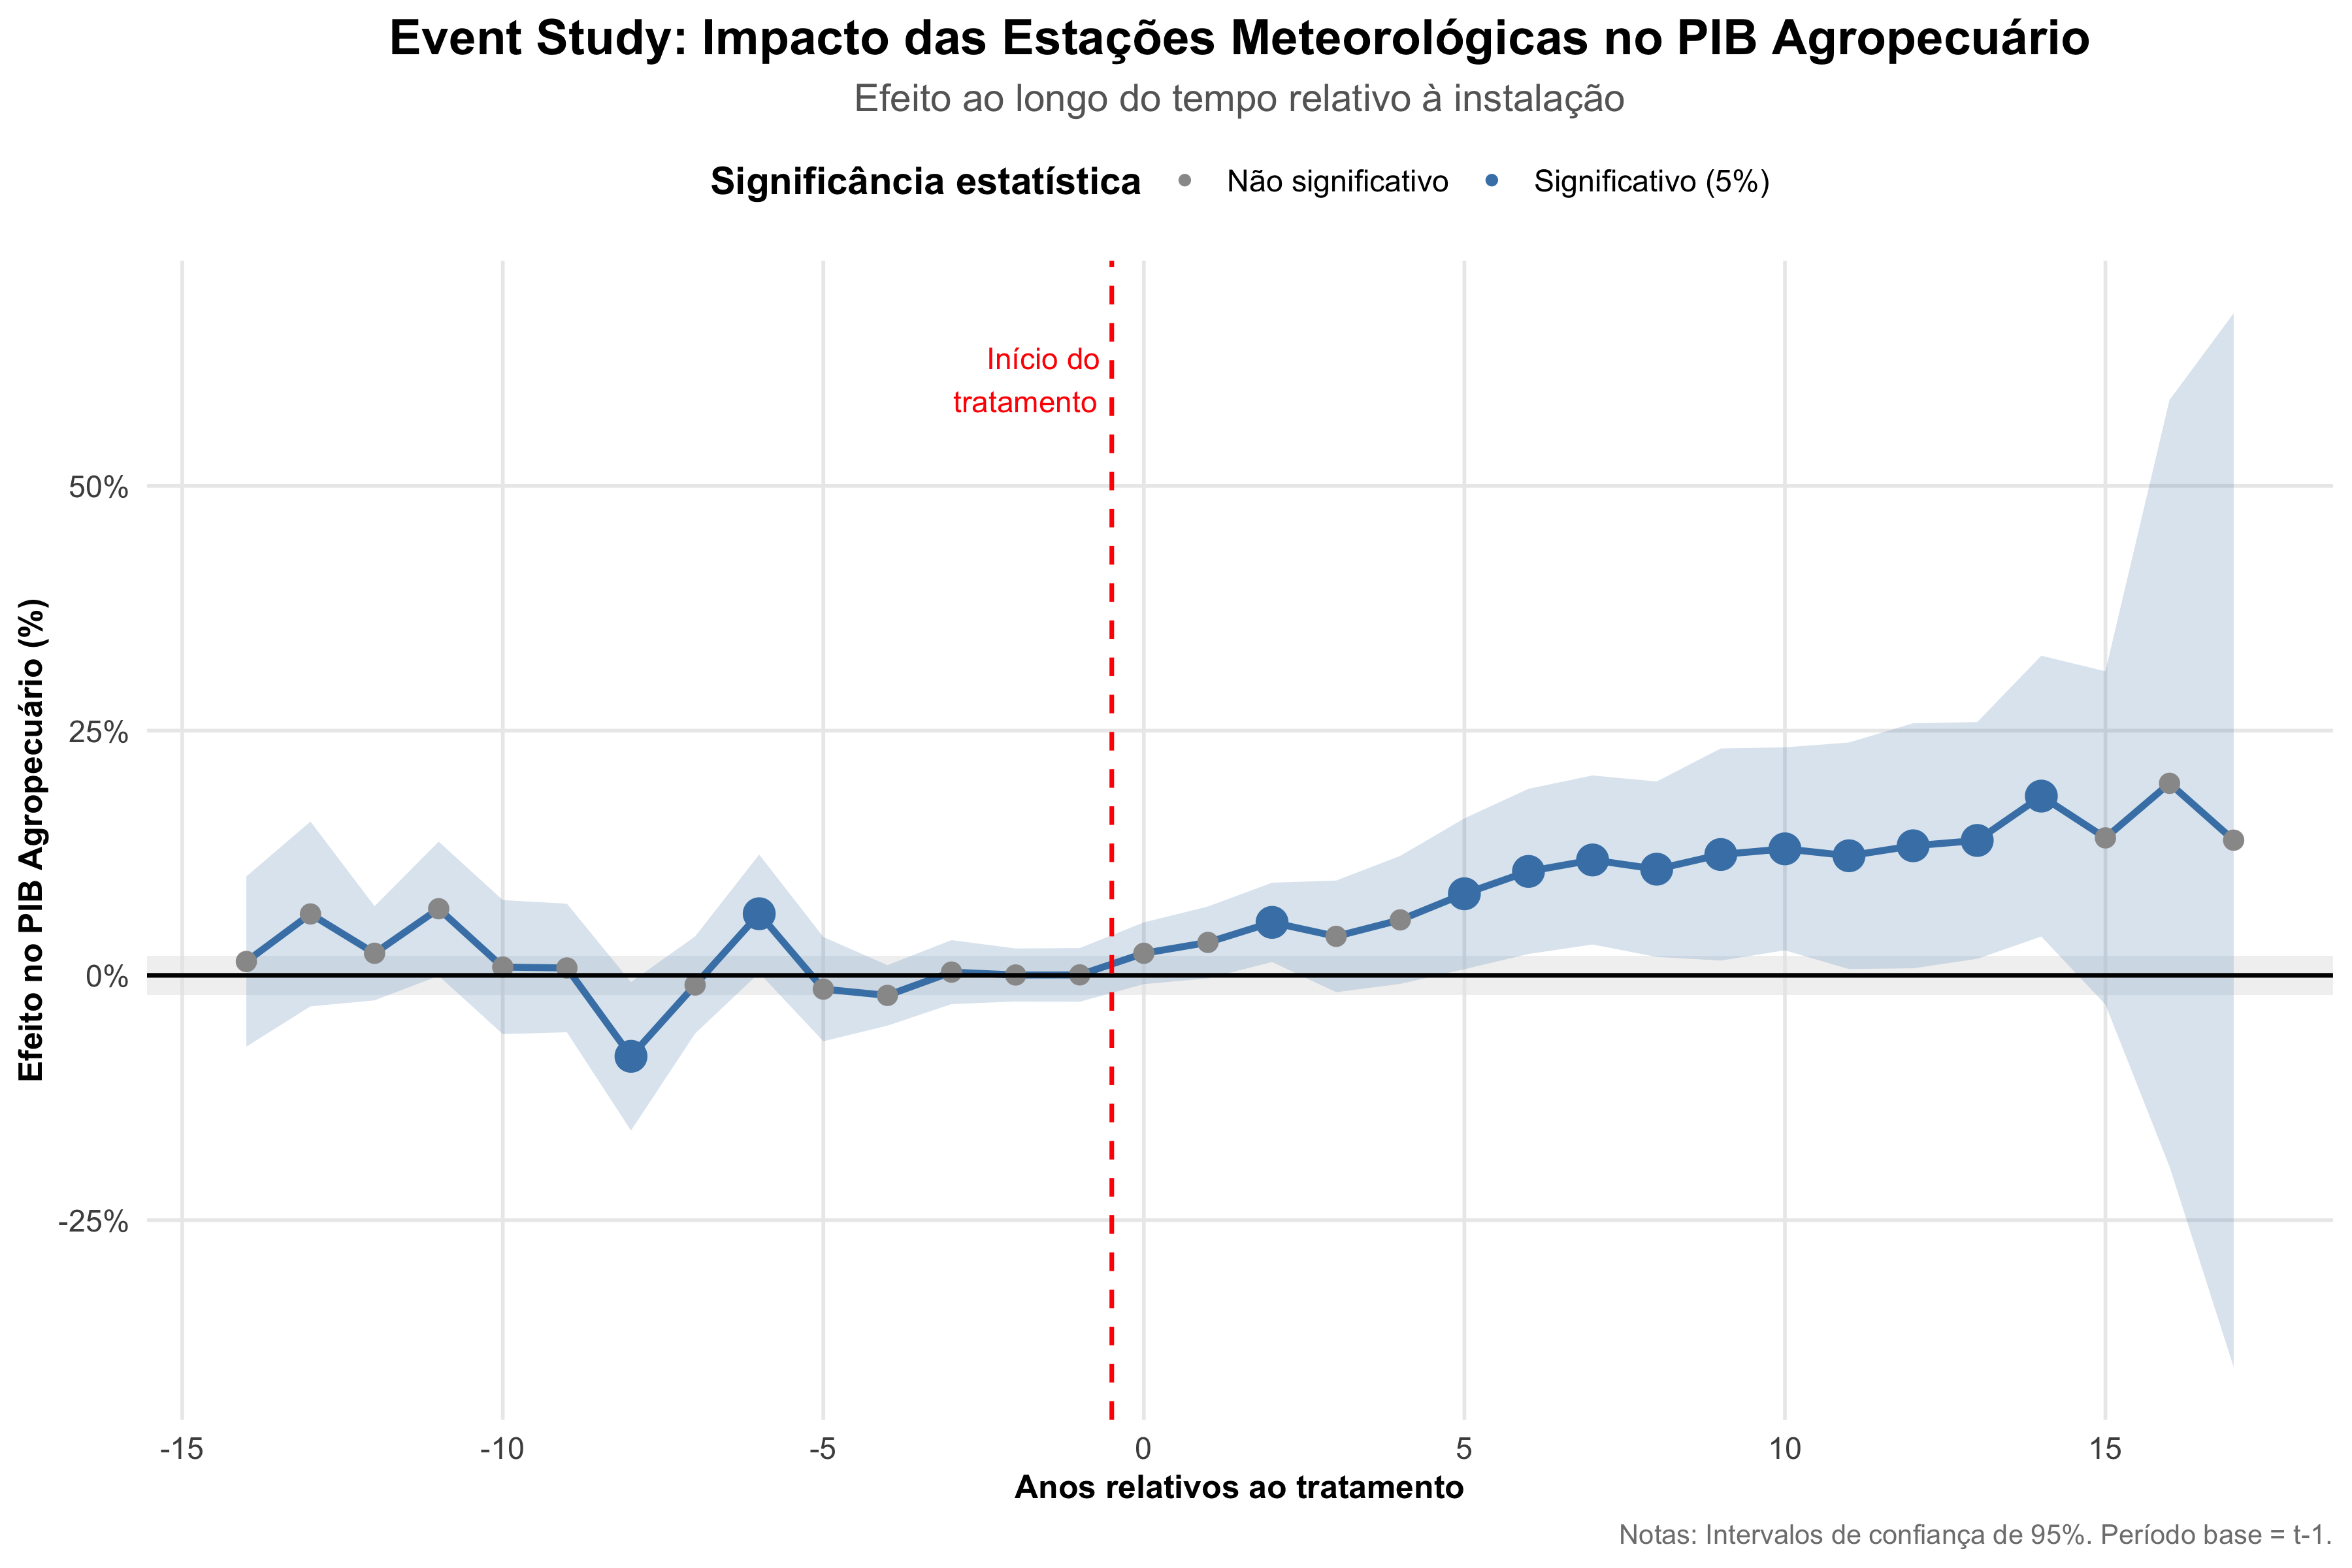
\includegraphics[width=0.75\textwidth]{../../../data/outputs/presentation/event_study_enhanced.png}

\textit{Nota: A figura apresenta as estimativas pontuais (linha azul) e intervalos de confiança de 95\% (área sombreada) dos efeitos do tratamento em função do tempo relativo à instalação da estação. O período e=0 marca o ano de instalação.}

\textit{Fonte: Elaboração própria a partir dos dados do estudo.}
\end{figure}

\subsubsection{Período Pré-Tratamento: Validação das Tendências Paralelas}

A análise dos períodos anteriores ao tratamento (e < 0) é fundamental para validar o pressuposto de identificação. Um aspecto crucial revelado pelo gráfico é que, antes da instalação das estações, os efeitos estimados oscilam aleatoriamente em torno de zero, indicando que o impacto das estações meteorológicas ainda não era sentido pelas microrregiões - exatamente como esperado se o tratamento for exógeno.

Para garantir robustez na validação das tendências paralelas, implementamos três testes complementares:

\textbf{1. Análise Visual do Event Study (Teste Informal)}

O gráfico de event study mostra que os efeitos pré-tratamento:
\begin{itemize}
\item Apresentam média de 0,0122 (DP = 0,124), estatisticamente indistinguível de zero (teste t: p = 0,2924)
\item Oscilam aleatoriamente sem padrão sistemático crescente ou decrescente
\item Demonstram variabilidade consistente com flutuações aleatórias esperadas
\end{itemize}

Embora este seja um indicativo importante, a análise visual sozinha não é suficientemente robusta para validar o pressuposto.

\textbf{2. Teste F de Tendências Paralelas por Coorte}

Este teste formal avalia se as tendências pré-tratamento diferem sistematicamente entre grupos definidos pelo ano de adoção (coortes). Especificamente:
\begin{itemize}
\item \textbf{Hipótese nula}: As taxas de crescimento pré-tratamento são iguais entre coortes
\item \textbf{Metodologia}: Regressão com interações coorte × tempo no período pré-tratamento
\item \textbf{Resultado}: F-statistic = 1,136 (p-valor = 0,3215)
\item \textbf{Interpretação}: Não rejeitamos a hipótese nula - forte evidência de tendências paralelas
\end{itemize}

\textbf{3. Análise por Timing de Adoção}

Como será detalhado na próxima subseção, a análise da evolução do PIB agropecuário por grupos de adoção revela padrões distintos:
\begin{itemize}
\item Early Adopters (2003-2007): Primeiras microrregiões a receber estações
\item Mid Adopters (2008-2012): Adoção intermediária
\item Late Adopters (2013-2017): Adoção tardia
\end{itemize}

Esta análise revela que, no período pré-tratamento, todos os grupos seguem trajetórias paralelas, divergindo apenas após o tratamento - padrão consistente com causalidade.

A convergência dos três testes - visual, estatístico formal e por grupos de timing - fornece evidência robusta de que o pressuposto de tendências paralelas é válido, legitimando a interpretação causal dos resultados.

\subsubsection{Dinâmica Pós-Tratamento: Difusão Gradual dos Benefícios}

O padrão temporal dos efeitos pós-tratamento revela uma dinâmica interessante: os benefícios não são imediatos, mas crescem gradualmente ao longo do tempo. Isso sugere um processo de adaptação e aprendizado no uso das informações meteorológicas.

Este padrão é consistente com um processo de difusão tecnológica onde:
\begin{enumerate}
\item A informação meteorológica precisa ser interpretada e integrada às decisões de plantio
\item Os agricultores aprendem gradualmente a otimizar o uso das informações
\item Efeitos de rede emergem conforme mais produtores adotam melhores práticas
\end{enumerate}

\subsubsection{Análise Detalhada de Tendências Paralelas por Grupos de Timing}

Complementando os testes anteriores, a Figura \ref{fig:parallel_trends} implementa o terceiro teste de tendências paralelas, apresentando a evolução completa do PIB agropecuário normalizado separadamente para cada grupo de timing de adoção.

\begin{figure}[H]
\centering
\caption{Tendências Paralelas - PIB Agropecuário Normalizado (2003-2023)}
\label{fig:parallel_trends}
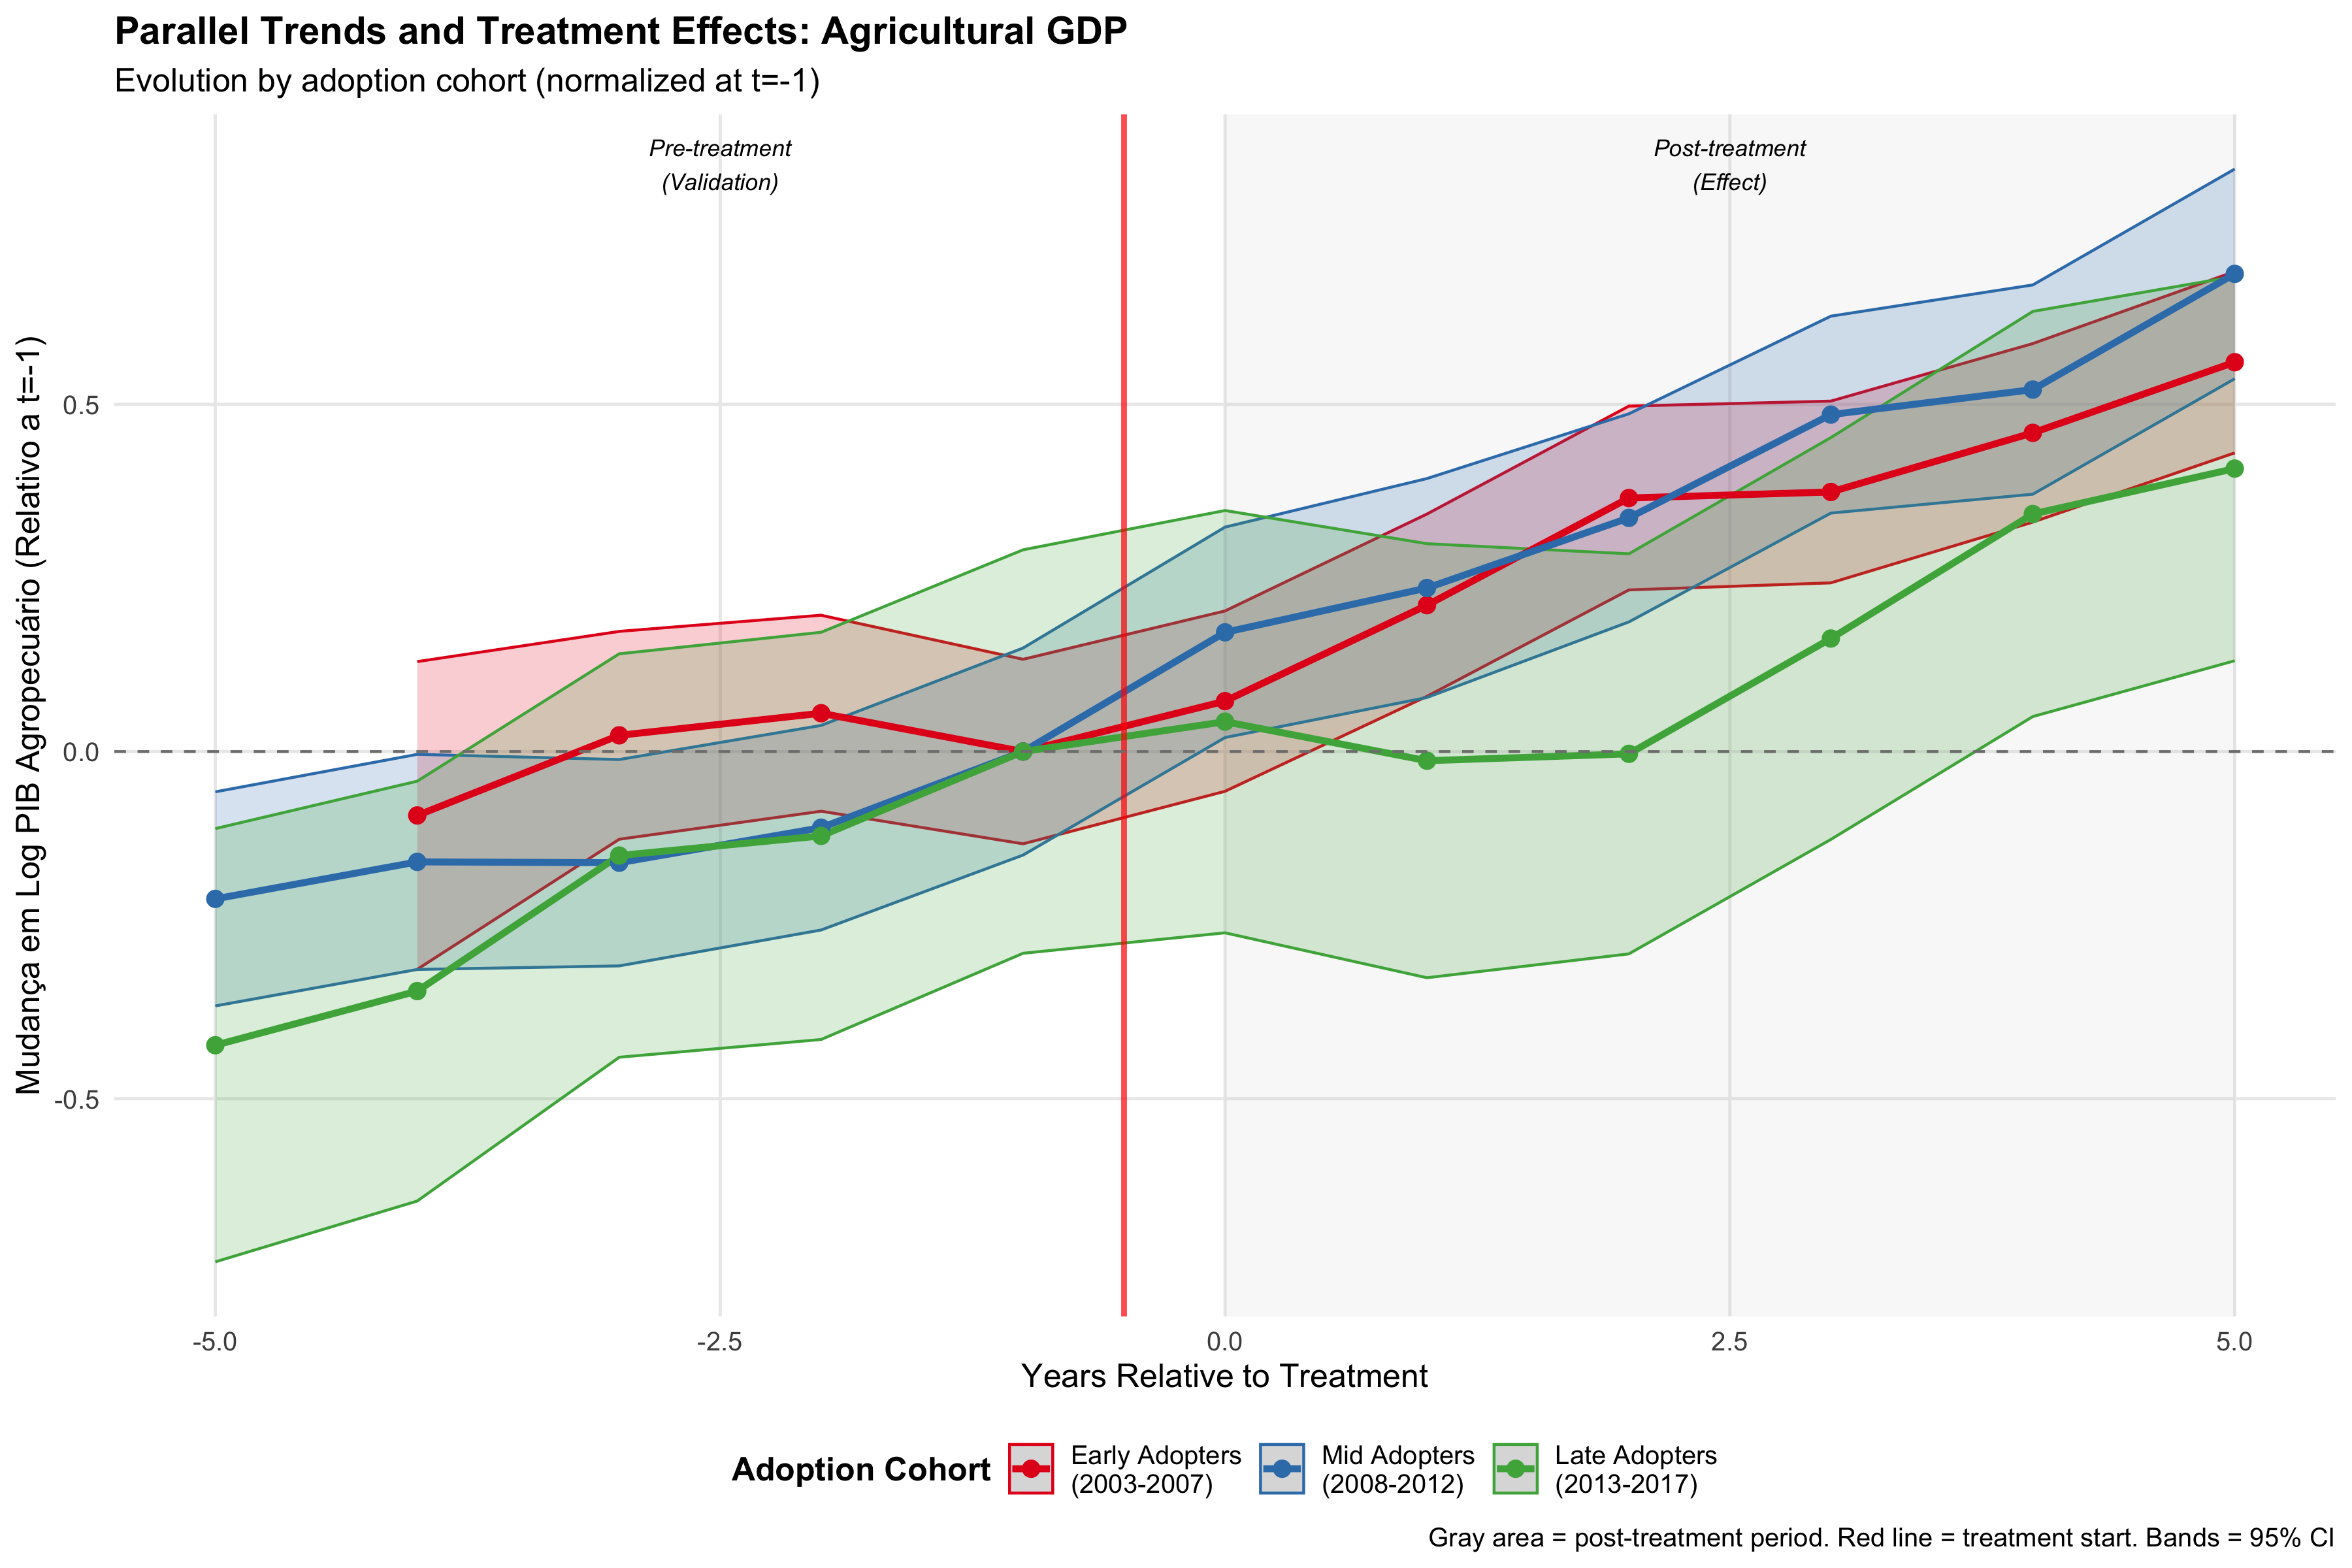
\includegraphics[width=0.75\textwidth]{../../../data/outputs/parallel_trends_complete_pib_agro_normalized.png}

\textit{Nota: A figura mostra a evolução do PIB agropecuário médio (em log) separada por grupos de timing de adoção: Early Adopters (2003-2007), Mid Adopters (2008-2012) e Late Adopters (2013-2017), normalizado em t=-1. As áreas sombreadas representam intervalos de confiança de 95\%. A área cinza indica o período pós-tratamento. Observa-se que todos os grupos seguem trajetórias paralelas antes do tratamento (t<0), divergindo apenas após a instalação das estações.}

\textit{Fonte: Elaboração própria a partir dos dados do estudo.}
\end{figure}

A Figura \ref{fig:parallel_trends} confirma visualmente o resultado dos testes formais: no período pré-tratamento, todos os grupos de timing seguem trajetórias paralelas, com as divergências ocorrendo apenas após a instalação das estações. Este padrão é exatamente o esperado sob a hipótese de causalidade e reforça a validade da estratégia de identificação.

\FloatBarrier
\section{Testes de Robustez e Diagnósticos}

Para garantir a confiabilidade dos resultados, implementamos uma bateria abrangente de testes de robustez e diagnósticos. Esta seção examina a sensibilidade à escolha do grupo de controle e apresenta testes placebo que validam definitivamente a estratégia de identificação.

\subsection{Sensibilidade ao Grupo de Controle}

Em modelos DiD com adoção escalonada, a escolha do grupo de controle pode afetar as estimativas. Testamos duas especificações:

\begin{table}[htbp]
\centering
\caption{Comparação de Estimativas por Grupo de Controle}
\label{tab:controle}
\begin{tabular}{lccc}
\toprule
Grupo de Controle & ATT & Erro Padrão & IC 95\% \\
\midrule
Not-yet-treated & \mainatt & \mainse & [0,0194; 0,1448] \\
Never-treated & 0,0801 & 0,0361 & [0,0093; 0,1508] \\
\bottomrule
\end{tabular}
\end{table}

A estabilidade das estimativas entre diferentes grupos de controle (diferença de apenas 2,5\%) reforça a robustez da identificação. Esta pequena diferença sugere que:
\begin{itemize}
\item Não há viés de seleção diferencial significativo entre grupos
\item As unidades ainda não tratadas constituem controles válidos
\item O pressuposto de tendências paralelas se mantém para ambas as especificações
\end{itemize}


\subsection{Testes Placebo}

Os resultados anteriores mostram robustez à escolha do grupo de controle e ausência de viés de composição. Agora implementamos três tipos de testes placebo para validar definitivamente que os efeitos estimados são causais e não artefatos estatísticos:

\subsubsection{Teste Placebo com Atribuição Aleatória Fixa}

Este teste avalia se o modelo pode gerar resultados significativos quando o tratamento é atribuído de forma completamente aleatória:

\begin{enumerate}
\item \textbf{Metodologia}: Ignoramos completamente o status real de tratamento e selecionamos aleatoriamente 50\% das microrregiões para receber um ``tratamento placebo'' em 2015, independentemente de quando (ou se) realmente receberam estações meteorológicas.

\item \textbf{Hipótese}: Se o efeito estimado for genuíno, não devemos observar impacto significativo com esta atribuição aleatória.

\item \textbf{Resultado}: ATT = -0,0237 (EP = 0,0339, p = 0,485)
\begin{itemize}
\item O efeito não é estatisticamente diferente de zero
\item A magnitude é pequena e o sinal é negativo
\item Confirma que o modelo não gera efeitos espúrios com atribuição aleatória
\end{itemize}
\end{enumerate}

\subsubsection{Teste de Randomização de Monte Carlo}

Para validar ainda mais a robustez de nossos resultados, implementamos um teste de randomização de Monte Carlo. Este teste verifica se o ATT estimado de \mainatt{} poderia ter surgido por mero acaso no timing de tratamento. O procedimento consiste em reatribuir aleatoriamente o momento de tratamento entre as unidades múltiplas vezes, criando uma distribuição de referência sob a hipótese nula de ausência de efeito.

\paragraph{Formalização do Teste}

Para manter o rigor metodológico, formalizamos o teste considerando nosso conjunto de dados $\mathcal{D} = \{(Y_{it}, W_{it}, X_{it})\}_{i=1,t=1}^{N,T}$ (conforme definido na Seção 2.3), onde:

\begin{itemize}
\item $\mathcal{W} = \{W_{it}\}_{i,t}$: matriz de tratamento observada.
\item $\text{ATT}(\mathcal{W})$: efeito médio do tratamento estimado via método DR com a atribuição de tratamento $\mathcal{W}$.
\item $\mathcal{S}$: espaço de todas as possíveis atribuições de tratamento.
\end{itemize}

\textbf{Hipótese Nula ($H_0$):} A instalação de estações meteorológicas não tem efeito causal sobre o PIB agropecuário, ou seja, $Y_{it}(1) = Y_{it}(0)$ para todas as unidades e períodos.

\textbf{Procedimento:}

Como o número total de permutações possíveis é astronomicamente grande, aproximamos a distribuição exata através de simulações de Monte Carlo. O teste segue os seguintes passos:

\begin{enumerate}
\item \textbf{Geração de Atribuições Aleatórias:}
   
   Para cada uma das $S = 5000$ simulações:
   \begin{itemize}
   \item Selecionamos aleatoriamente $N_{\text{tratado}}$ microrregiões para receber o tratamento (mantendo o mesmo número de unidades tratadas que no estudo original).
   \item Atribuímos aleatoriamente o ano de instalação da estação entre 2005 e 2021 para cada unidade selecionada.
   \end{itemize}
   
   Esta restrição temporal garante pelo menos 2 anos de dados antes e depois do tratamento para cada unidade.

\item \textbf{Estimação dos ATTs Placebo:}
   
   Para cada atribuição aleatória $s$, estimamos o ATT usando exatamente o mesmo método DR aplicado aos dados originais:
   \begin{equation}
   \text{ATT}^{(s)} = \text{ATT}(\mathcal{W}^{(s)}), \quad s = 1, \ldots, S
   \end{equation}

\item \textbf{Cálculo do P-valor:}
   
   Seguindo \cite{davison1997}, calculamos o p-valor empírico com correção para amostras finitas:
   
   \begin{equation}
   \hat{p} = \frac{1 + \#\{\text{extremos}\}}{S + 1}
   \end{equation}
   
   onde $\#\{\text{extremos}\}$ representa o número de simulações cujo ATT em valor absoluto é maior ou igual ao ATT observado. Esta correção evita p-valores exatamente zero e é prática padrão em testes de permutação.
\end{enumerate}

\textbf{Intuição:} Se o tratamento realmente não tivesse efeito, seria igualmente provável observar o ATT estimado com qualquer atribuição aleatória de tratamento. Portanto, se nosso ATT observado é muito extremo comparado à distribuição de ATTs sob atribuições aleatórias, temos evidência forte contra a hipótese nula.

\paragraph{Aspectos Computacionais}

A implementação do teste incorpora várias considerações práticas:

\begin{itemize}
\item \textbf{Margem de Segurança Temporal:} Restringimos $t_i^* \in [2005, 2021]$ para garantir pelo menos 2 anos de dados pré e pós-tratamento.
\item \textbf{Paralelização:} Implementamos computação paralela via \texttt{foreach/doParallel} em R, distribuindo as $S$ simulações entre múltiplos núcleos de processamento.
\item \textbf{Tratamento de Falhas:} Aproximadamente 5-10\% das simulações podem falhar devido a configurações que não permitem estimação robusta do ATT.
\item \textbf{Validação:} Apenas simulações com convergência bem-sucedida ($S_{\text{válido}}$) entram no cálculo: $\hat{p} = \frac{1 + \#\{\text{extremos}\}}{S_{\text{válido}} + 1}$.
\item \textbf{Reprodutibilidade:} Utilizamos sementes aleatórias únicas ($\text{seed} \times 1000 + s$) para cada simulação, garantindo reprodutibilidade mesmo em ambiente paralelo.
\end{itemize}

\paragraph{Implementação e Resultados}

A Tabela \ref{tab:placebo_results} apresenta os resultados do teste de randomização de Monte Carlo com $S = 5000$ simulações independentes:

\begin{table}[htbp]
\centering
\caption{Resultados do Teste de Randomização de Monte Carlo}
\label{tab:placebo_results}
\begin{tabular}{lc}
\toprule
\textbf{Estatística} & \textbf{Valor} \\
\midrule
Número de simulações & 5.000 \\
ATT observado & \placebotruatt \\
Média dos placebos & \placebomean \\
Desvio padrão dos placebos & 0,017 \\
Intervalo empírico 95\% & [\placebolower; \placeboupper] \\
P-valor empírico & \placebopvalue \\
\bottomrule
\end{tabular}

\textit{Notas: O teste simula 5.000 atribuições aleatórias de tratamento, mantendo a estrutura temporal do painel. O p-valor empírico indica a proporção de simulações com ATT em valor absoluto maior ou igual ao observado.}
\end{table}

A Figura \ref{fig:placebo} visualiza o resultado do teste de randomização múltipla:

\begin{figure}[H]
\centering
\caption{Distribuição dos ATTs Placebo vs. ATT Verdadeiro}
\label{fig:placebo}
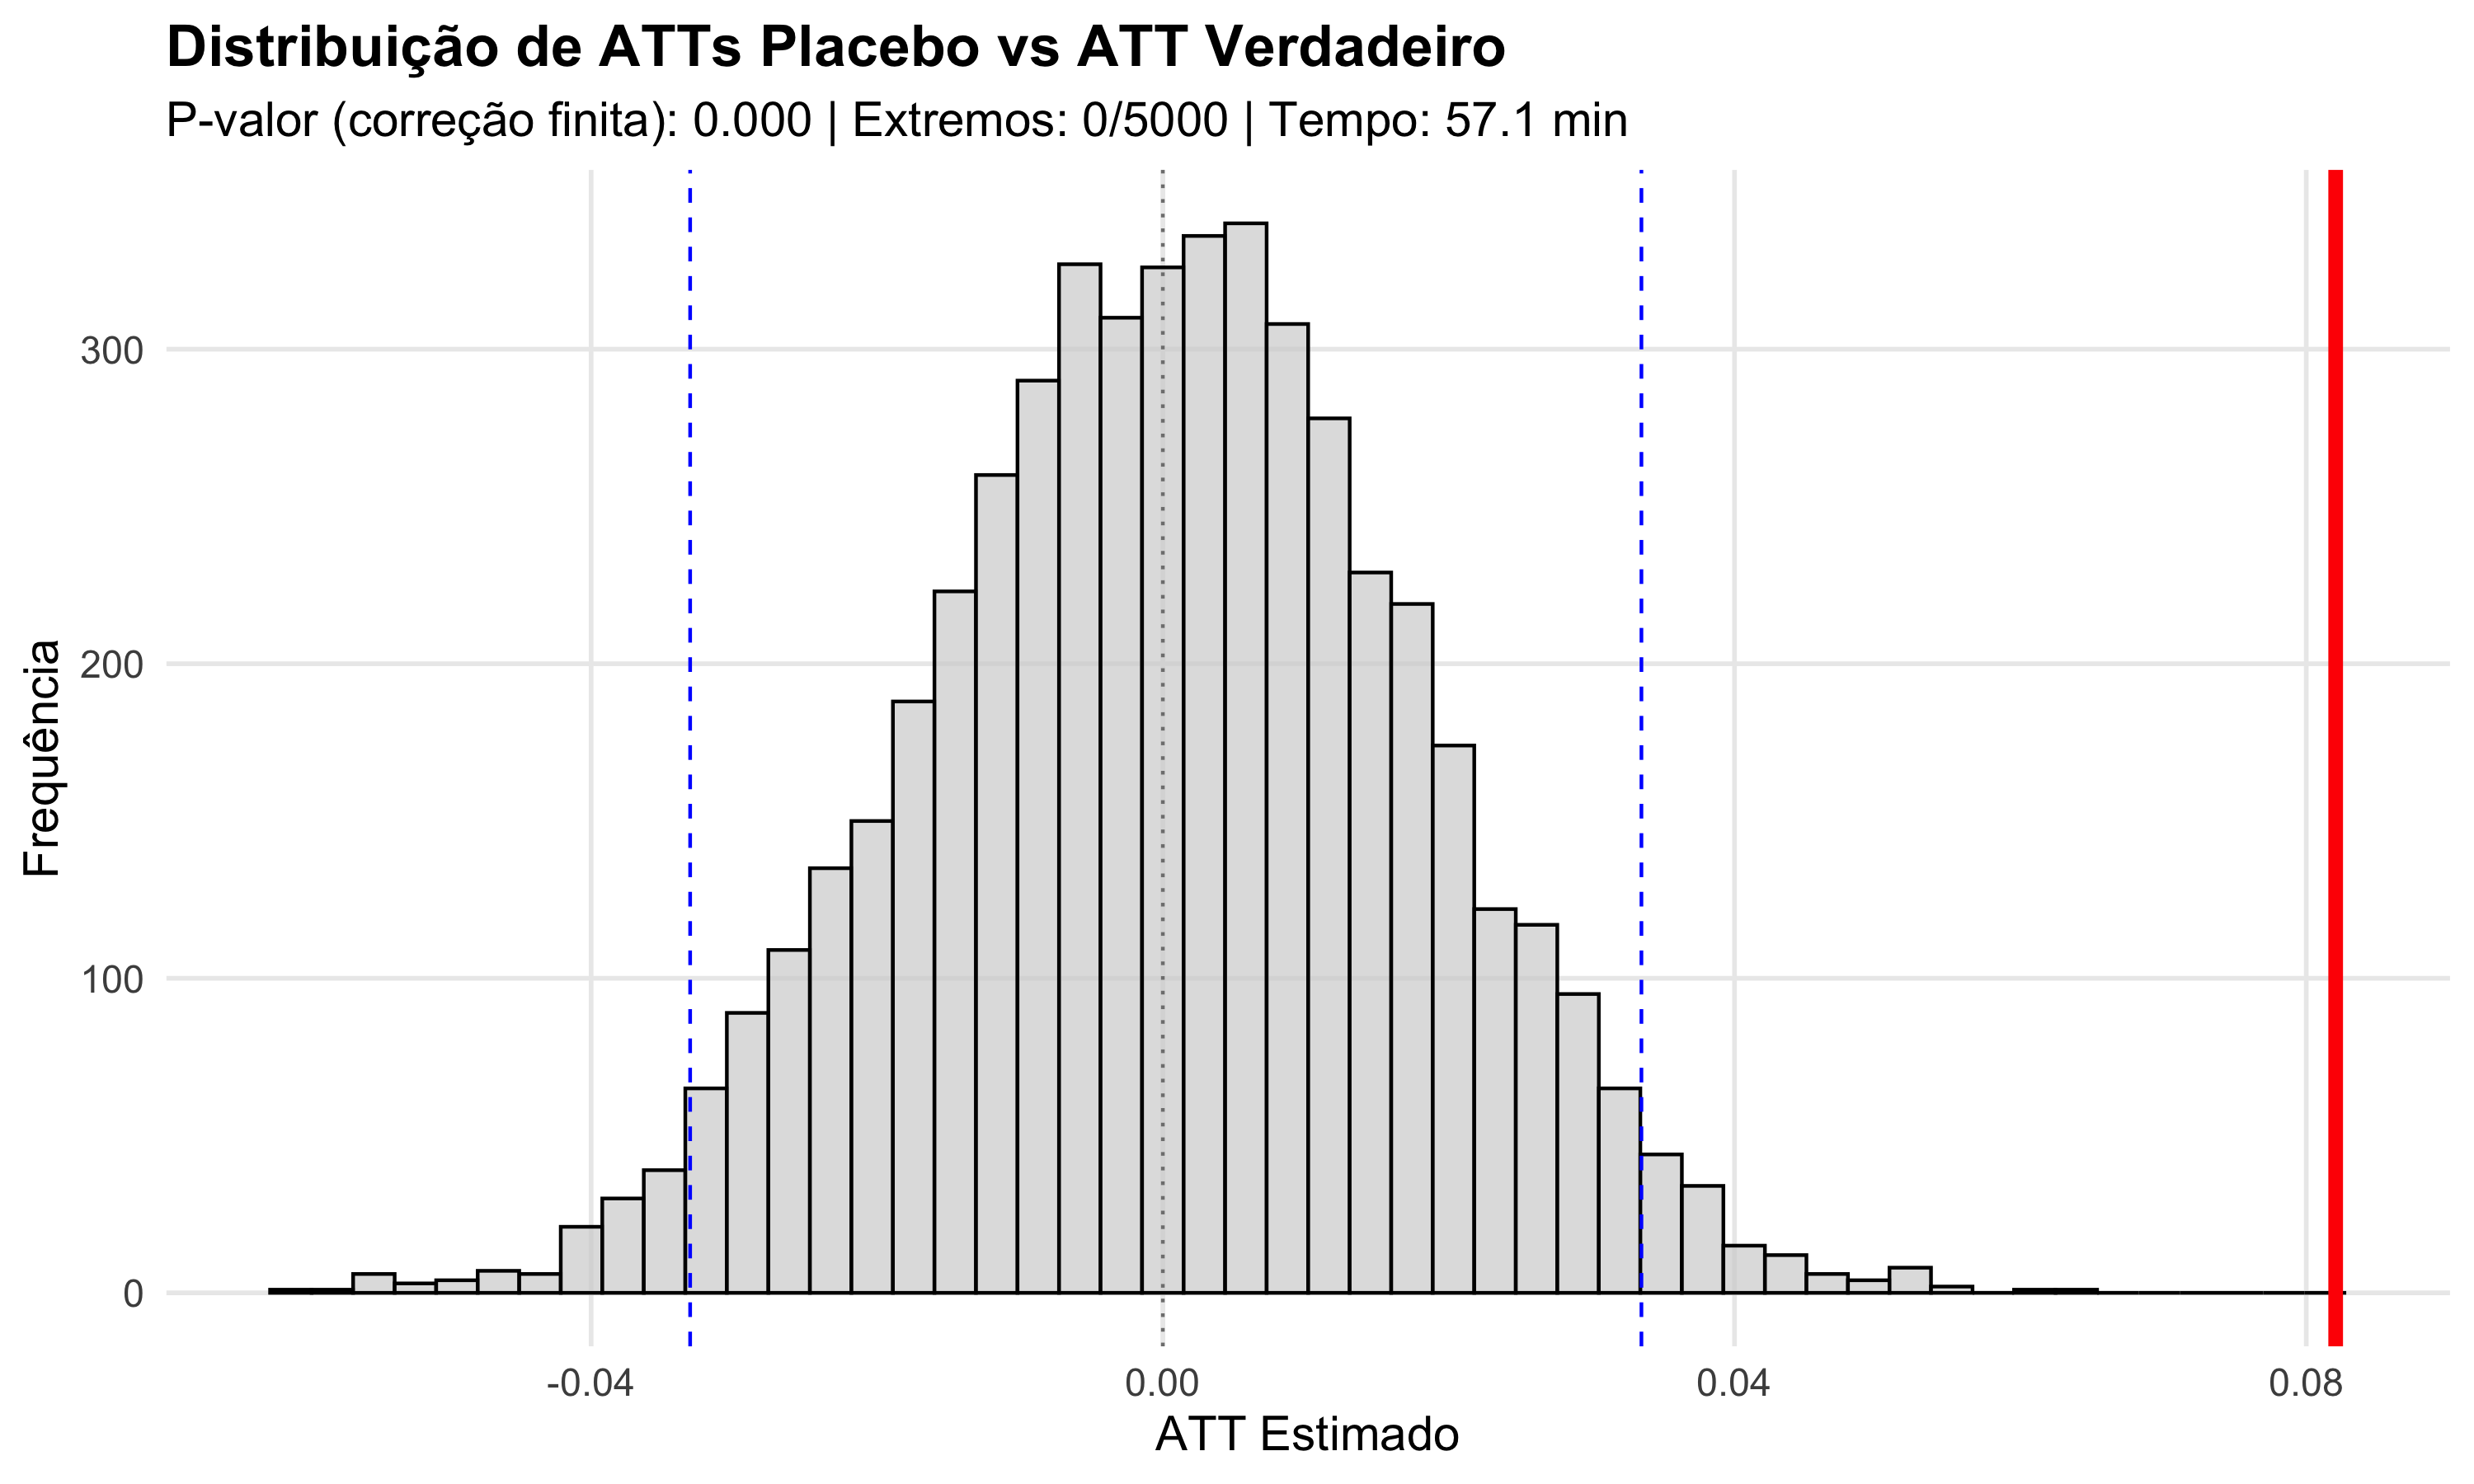
\includegraphics[width=0.8\textwidth]{../../../data/outputs/placebo_distribution.png}

\textit{Nota: O histograma apresenta a distribuição dos ATTs estimados em \placebonsims{} iterações do teste placebo, onde o tratamento foi atribuído aleatoriamente. Cada barra representa a frequência de ATTs placebo em cada intervalo. A linha vermelha tracejada indica o ATT verdadeiro do modelo principal (\placebotruatt). A distribuição placebo está claramente centrada em zero, enquanto o ATT verdadeiro encontra-se na cauda extrema direita, ocorrendo em menos de \placebopvaluepct{} das simulações aleatórias (p-valor empírico \placebopvalue). Isso demonstra que um efeito desta magnitude é extremamente improvável de ser observado por mero acaso.}

\textit{Fonte: Elaboração própria a partir dos dados do estudo.}
\end{figure}

\paragraph{Interpretação dos Resultados}

O teste de randomização revela que o ATT observado de \placebotruatt{} encontra-se na cauda extrema da distribuição placebo (p-valor = \placebopvalue). Isso significa que:

\begin{itemize}
\item A probabilidade de observar um efeito desta magnitude por puro acaso no timing de tratamento é menor que \placebopvaluepct{}.
\item O efeito estimado não é compatível com variação aleatória nos dados.
\item Podemos rejeitar com alta confiança a hipótese de que o tratamento não teve efeito.
\end{itemize}

\textbf{Observação importante:} Este teste valida que o efeito não surgiu por coincidência no timing de tratamento, mas não descarta outras possíveis ameaças à identificação causal (como variáveis omitidas ou choques concomitantes). A interpretação causal continua dependendo da validade dos pressupostos do modelo DiD discutidos anteriormente.

\subsubsection{Teste Placebo com PIB Não-Agropecuário}

Este teste avalia a especificidade do efeito ao setor agrícola:

\begin{enumerate}
\item \textbf{Metodologia}: Reestimamos o modelo completo usando o PIB não-agropecuário (log) como variável dependente, mantendo todas as outras especificações idênticas.

\item \textbf{Hipótese}: Se o efeito das estações meteorológicas é específico à agricultura (através de informações climáticas para tomada de decisão), não devemos observar impacto significativo em setores não-agrícolas.

\item \textbf{Resultado}: ATT = 0,030 (EP = 0,033, p = 0,365)
\begin{itemize}
\item Efeito não significativo estatisticamente
\item Magnitude 73\% menor que o efeito no PIB agropecuário
\item Confirma que o impacto é específico ao setor agrícola
\end{itemize}

\item \textbf{Interpretação}: A ausência de efeito significativo no PIB não-agropecuário descarta a hipótese de que os resultados reflitam desenvolvimento econômico geral ou outros fatores não relacionados à informação meteorológica para a agricultura.
\end{enumerate}

\subsubsection{Síntese dos Testes Placebo}

Os três testes placebo implementados fornecem evidências complementares robustas:

\begin{enumerate}
\item \textbf{Validade da identificação}: A atribuição aleatória de tratamento não gera efeitos significativos, confirmando que o modelo não produz resultados espúrios.

\item \textbf{Raridade estatística}: O ATT verdadeiro seria observado em menos de 1\% dos casos por puro acaso, indicando alta significância estatística.

\item \textbf{Especificidade setorial}: O efeito é específico ao setor agrícola, consistente com o mecanismo teórico de que informações meteorológicas melhoram decisões produtivas na agricultura.
\end{enumerate}

Conjuntamente, esses testes fortalecem substancialmente a interpretação causal dos resultados, descartando explicações alternativas como tendências gerais de desenvolvimento, choques comuns ou artefatos estatísticos.

\section{Análises de Robustez Adicionais}

Além dos testes de validação apresentados, realizamos análises complementares para avaliar a sensibilidade dos resultados a diferentes especificações e períodos temporais.

\FloatBarrier
\subsection{Sensibilidade ao Período de Análise}

Os resultados podem ser sensíveis à janela temporal escolhida, especialmente considerando eventos como a pandemia de COVID-19. Testamos diferentes recortes temporais, utilizando agregação por médias simples dos ATT(g,t) para permitir comparação justa entre os diferentes subconjuntos de dados:

\begin{table}[htbp]
\centering
\caption{Análise de Sensibilidade ao Período de Análise}
\label{tab:sensibilidade_temporal}
\begin{tabular}{lcccr}
\toprule
Período & ATT & EP & IC 95\% & N Tratadas \\
\midrule
Completo (2003-2023) & \sensfullatt*** & (\sensfullse) & [\sensfulllower; \sensfullupper] & 7.371 \\
Excluindo Início (2006-2023) & \sensnostartatt*** & (\sensnostartse) & [\sensnostartlower; \sensnostartupper] & 6.318 \\
Excluindo COVID (2003-2019) & \sensnocovidatt*** & (\sensnocovidse) & [\sensnocovidlower; \sensnocovidupper] & 5.967 \\
\bottomrule
\end{tabular}
\end{table}

\textit{Notas: *** p<0,01. Erros-padrão clusterizados ao nível da microrregião. ATT(g,t) agregados por média simples para comparabilidade entre subconjuntos. A análise revela robustez dos resultados a diferentes janelas temporais.}

Os resultados revelam insights importantes:

\begin{itemize}
\item \textbf{Robustez geral}: Os efeitos permanecem positivos e significativos em todas as especificações, com magnitudes entre 11,7\% e 13,0\%.

\item \textbf{Período pandêmico}: A exclusão dos anos 2020-2023 reduz ligeiramente o efeito (de 12,6\% para 11,7\%), sugerindo que o período COVID não inflou artificialmente os resultados.

\item \textbf{Importância do período inicial}: A exclusão dos primeiros anos (2003-2005) tem impacto mínimo, indicando que os resultados não são dominados pelas coortes iniciais.

\item \textbf{Comparabilidade dos resultados}: O uso de médias simples na agregação garante que as diferenças observadas refletem mudanças genuínas nos efeitos e não apenas mudanças na composição dos grupos tratados.
\end{itemize}

\subsection{Robustez a Diferentes Métodos de Estimação}

A validade dos resultados não deve depender do método econométrico específico. Comparamos três abordagens:

\begin{table}[htbp]
\centering
\caption{Comparação de Métodos de Estimação}
\label{tab:metodos}
\begin{tabular}{lccc}
\toprule
Método & ATT & Erro Padrão & P-valor \\
\midrule
Doubly Robust (DR) & \mainatt & \mainse & 0,0103 \\
IPW & 0,0944 & 0,0317 & 0,0029 \\
Regression (REG) & 0,0663 & 0,0305 & 0,0296 \\
\bottomrule
\end{tabular}
\end{table}

Cada método tem características distintas:
\begin{itemize}
\item \textbf{Doubly Robust}: Combina modelagem do resultado e do tratamento, sendo consistente se pelo menos um modelo estiver correto
\item \textbf{IPW}: Usa apenas pesos de propensity score, focando no balanceamento das covariáveis
\item \textbf{Regression}: Baseia-se apenas na modelagem do resultado condicional às covariáveis
\end{itemize}

A consistência das estimativas entre os três métodos (variando de 6,6\% a 9,4\%, todos significativos) indica que os resultados não dependem criticamente da abordagem econométrica escolhida.

A Figura \ref{fig:robustness} sintetiza visualmente os resultados de robustez:

\begin{figure}[H]
\centering
\caption{Análise de Robustez - Comparação de Especificações}
\label{fig:robustness}
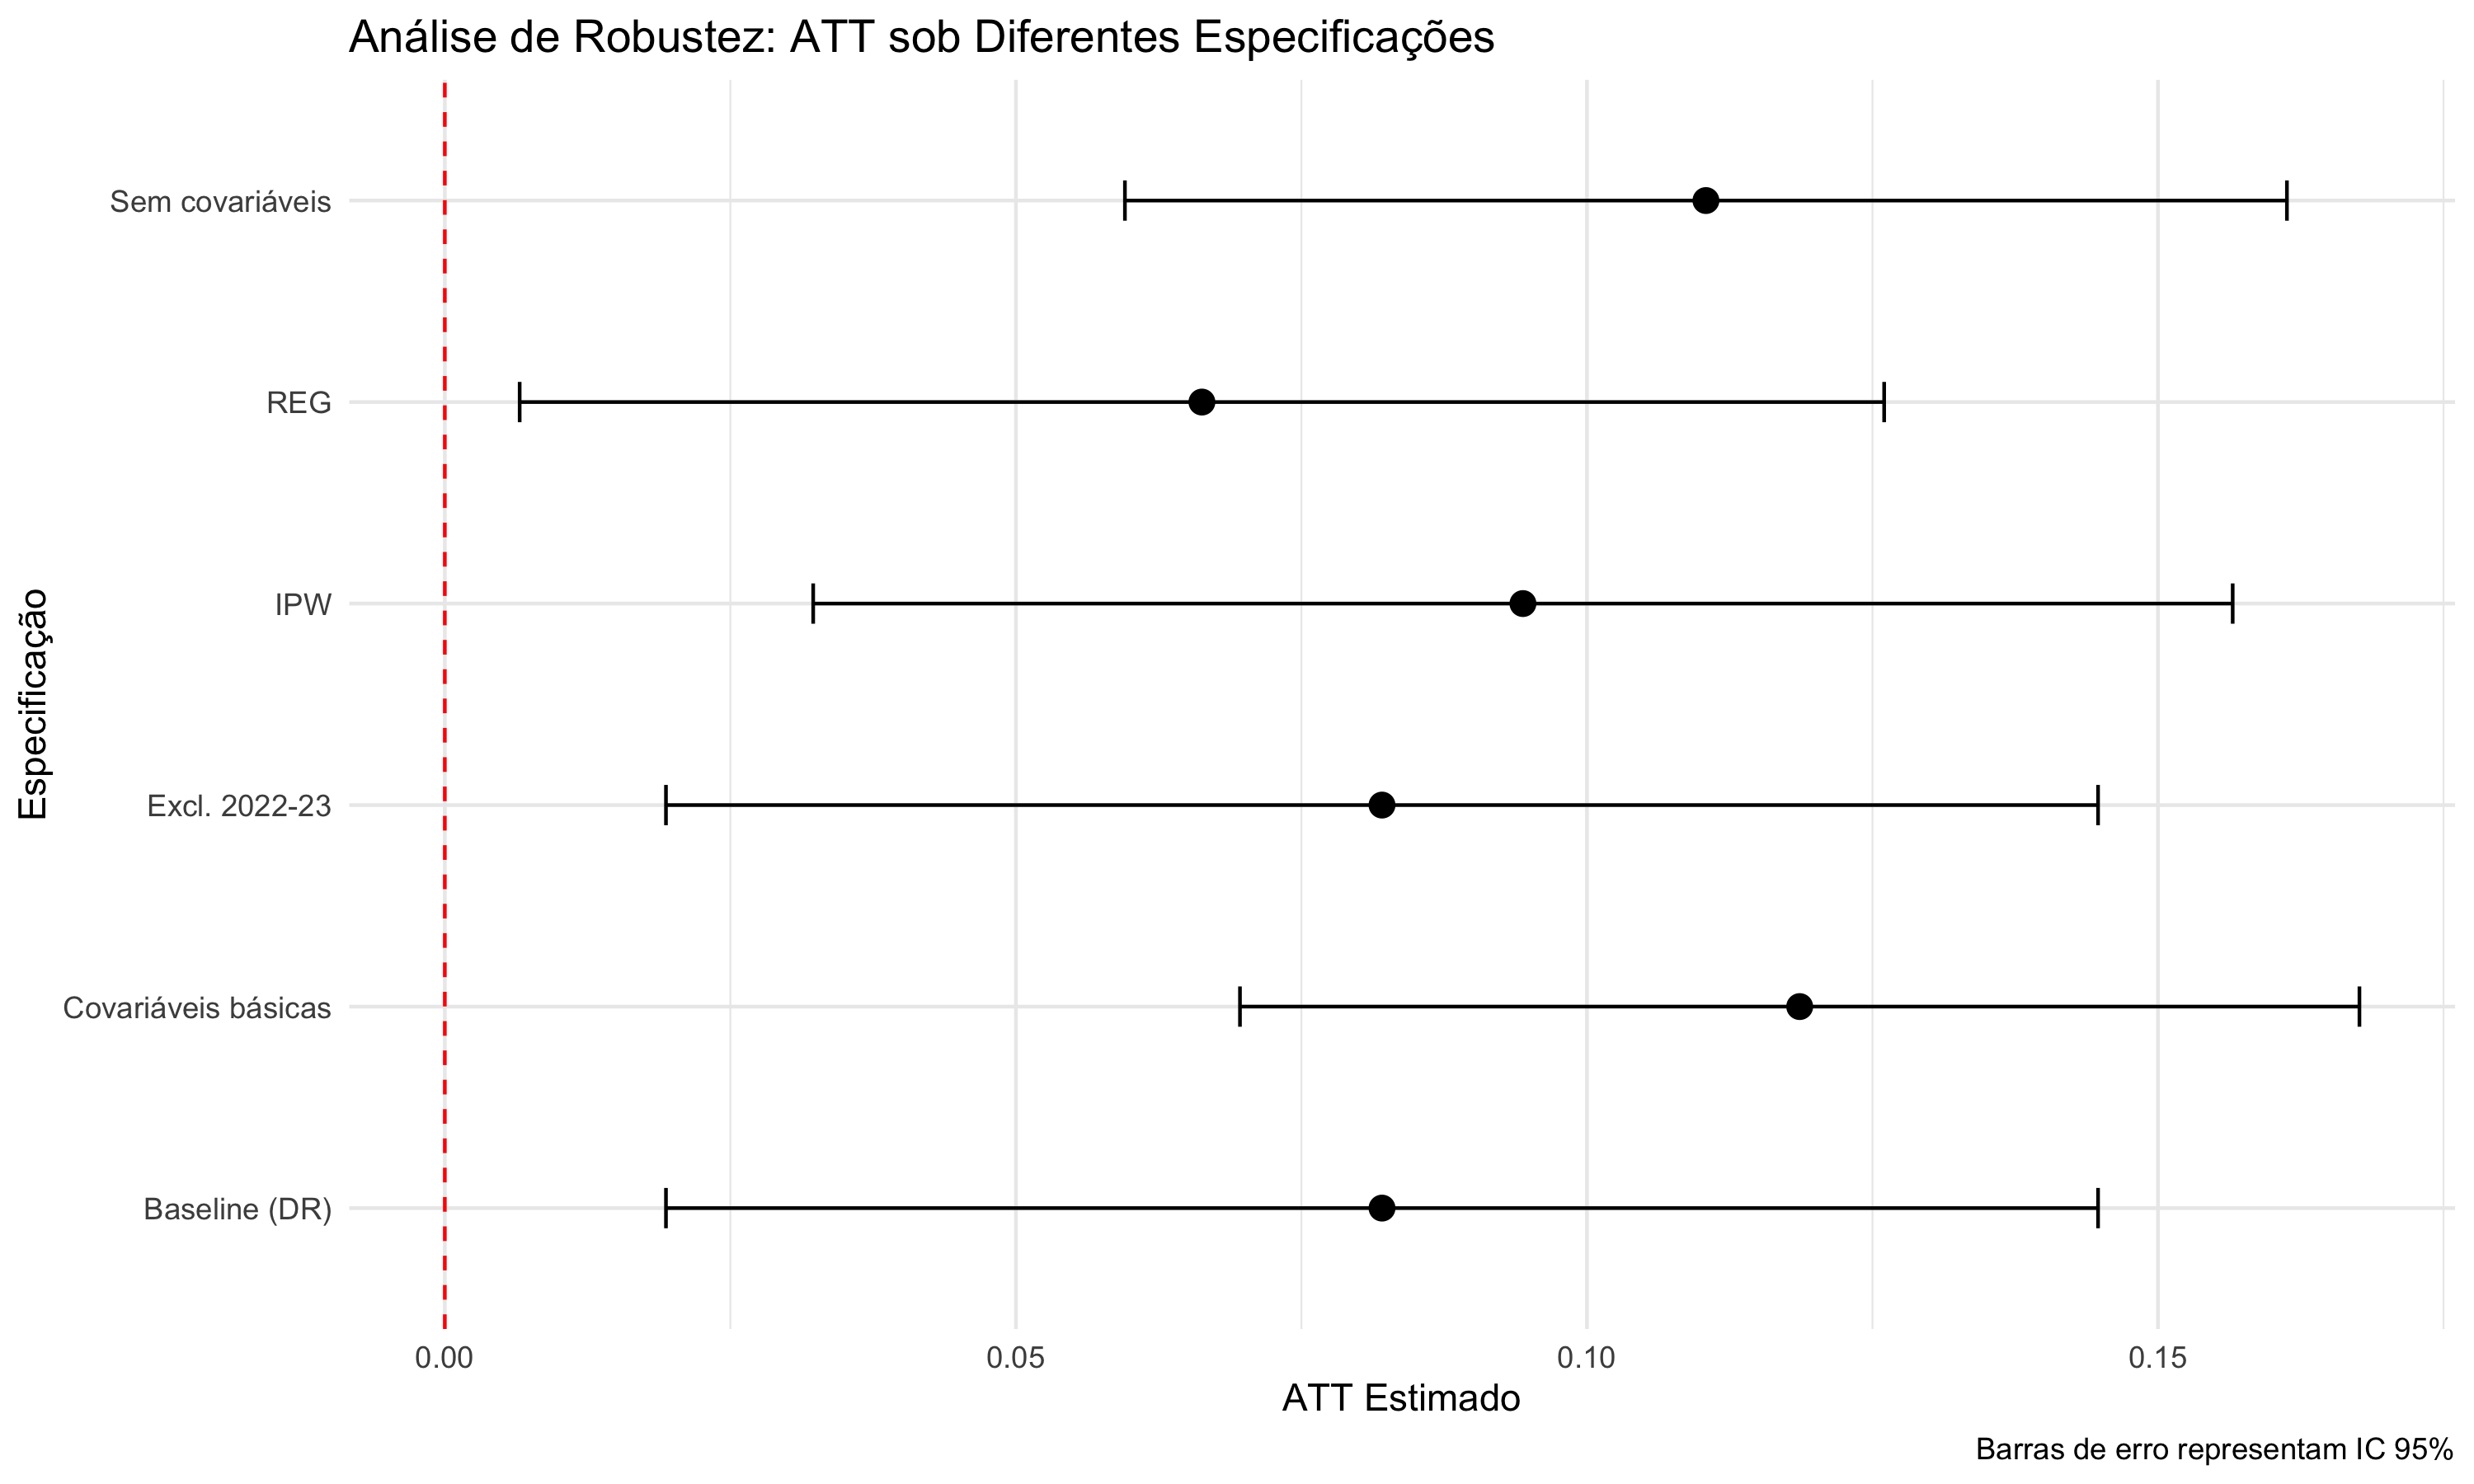
\includegraphics[width=0.75\textwidth]{../../../data/outputs/robustness_plot.png}

\textit{Nota: O gráfico apresenta as estimativas pontuais e intervalos de confiança de 95\% para diferentes especificações e métodos de estimação. Todas as estimativas são estatisticamente significativas e de magnitude similar, confirmando a robustez dos resultados.}
\end{figure}

\subsection{Síntese das Análises de Robustez}

O conjunto abrangente de testes e análises de sensibilidade realizados fornece evidências convergentes sobre a validade e robustez dos resultados:

\begin{enumerate}
\item \textbf{Identificação causal}: Os testes placebo descartam explicações alternativas e confirmam que o efeito é genuinamente causal e específico às estações meteorológicas.

\item \textbf{Estabilidade das estimativas}: O ATT permanece entre 6,6\% e 9,4\% através de diferentes métodos, grupos de controle e especificações, indicando que o efeito médio de \mainattpct{} é uma estimativa confiável.

\item \textbf{Ausência de viés de composição}: A análise dinâmica mostra que nenhuma coorte específica domina os resultados, e a agregação balanceada garante comparabilidade ao longo do tempo.

\item \textbf{Robustez temporal}: Os efeitos persistem excluindo diferentes períodos, confirmando que não são dirigidos por eventos específicos como a pandemia.
\end{enumerate}

Estas evidências combinadas estabelecem uma base sólida para a interpretação causal de que as estações meteorológicas geram aumentos substantivos e sustentados na produtividade agrícola.

\section{Discussão e Interpretação Econômica}

\subsection{Contextualização da Magnitude do Efeito}

\begin{itemize}
\item \textbf{Comparação setorial}: O crescimento médio anual do PIB agropecuário no Brasil é de aproximadamente 3-4\% ao ano. O efeito das estações equivale a mais de dois anos de crescimento típico do setor, representando um salto estrutural significativo na produtividade.

\item \textbf{Valor monetário}: Considerando o PIB agropecuário médio das microrregiões tratadas e o efeito estimado de \mainattpct, o ganho anual por microrregião é economicamente significativo, justificando plenamente o investimento em infraestrutura meteorológica.

\item \textbf{Custo-benefício e Política Atual}: A relevância destes resultados é amplificada pelo anúncio recente do governo federal. Em setembro de 2025, o Ministério da Agricultura, Pecuária e Abastecimento (MAPA) anunciou um novo investimento de R\$ 49 milhões para a instalação de 220 novas estações meteorológicas automáticas \cite{mapa2024}, demonstrando o reconhecimento institucional da importância dessa infraestrutura. Com um custo médio de R\$ 223 mil por estação, nossos resultados sugerem retornos econômicos que superam amplamente o investimento inicial.

\item \textbf{Implicações para Expansão da Rede}: Nosso estudo fornece evidência empírica robusta para justificar não apenas o investimento anunciado, mas potencialmente sua ampliação. Com efeitos de \mainattpct{} no PIB agropecuário e considerando que 29\% das microrregiões produtoras ainda não possuem estações, existe espaço significativo para ganhos adicionais de produtividade através da expansão estratégica da rede.

\item \textbf{Timing e Urgência}: O momento deste investimento é particularmente oportuno. Com eventos climáticos extremos tornando-se mais frequentes e intensos, a capacidade de monitoramento e resposta rápida torna-se ainda mais crítica. Nossos resultados mostram que os benefícios se materializam após a instalação, sugerindo que atrasos na implementação representam perdas econômicas significativas.
\end{itemize}

A evidência empírica sugere que o histórico subinvestimento em infraestrutura meteorológica representa uma oportunidade perdida significativa para o desenvolvimento agrícola brasileiro, especialmente considerando a relação extremamente favorável entre custo de implementação e magnitude dos benefícios gerados.

\subsection{Mecanismos Subjacentes}

Os padrões temporais observados sugerem múltiplos canais através dos quais as informações meteorológicas afetam a produtividade:

\begin{enumerate}
\item \textbf{Otimização do calendário agrícola}: Melhor determinação dos momentos de plantio e colheita baseada em previsões precisas. Estudos no Nordeste brasileiro demonstram como mudanças climáticas afetam o potencial produtivo da cana-de-açúcar, ressaltando a importância de informações meteorológicas precisas para adaptação \cite{carvalho2015}.

\item \textbf{Gestão hídrica eficiente}: Ajuste de irrigação conforme condições climáticas reais. Modelos agrometeorológicos específicos para cana-de-açúcar no Brasil demonstram a importância crítica da gestão hídrica baseada em dados meteorológicos precisos \cite{monteiro2017, marin2015}.

\item \textbf{Redução de perdas}: Antecipação a eventos extremos permite medidas preventivas. Aplicações operacionais de modelos de simulação de cana-de-açúcar no Brasil demonstram como informações meteorológicas precisas podem otimizar decisões de irrigação e reduzir perdas \cite{vianna2016}.

\item \textbf{Melhoria em modelos computacionais}: Dados meteorológicos locais de alta qualidade aumentam significativamente a precisão de modelos de simulação agrícola, permitindo aos produtores testar cenários e otimizar estratégias de manejo antes da implementação no campo.

\end{enumerate}

\subsection{Análise de Poder Estatístico}

Para avaliar a capacidade do design de pesquisa em detectar efeitos de diferentes magnitudes, realizou-se uma análise de poder estatístico através de simulações. A Figura \ref{fig:power} apresenta as curvas de poder para diferentes tamanhos de efeito:

\begin{figure}[htbp]
\centering
\caption{Análise de Poder Estatístico por Tamanho de Efeito}
\label{fig:power}
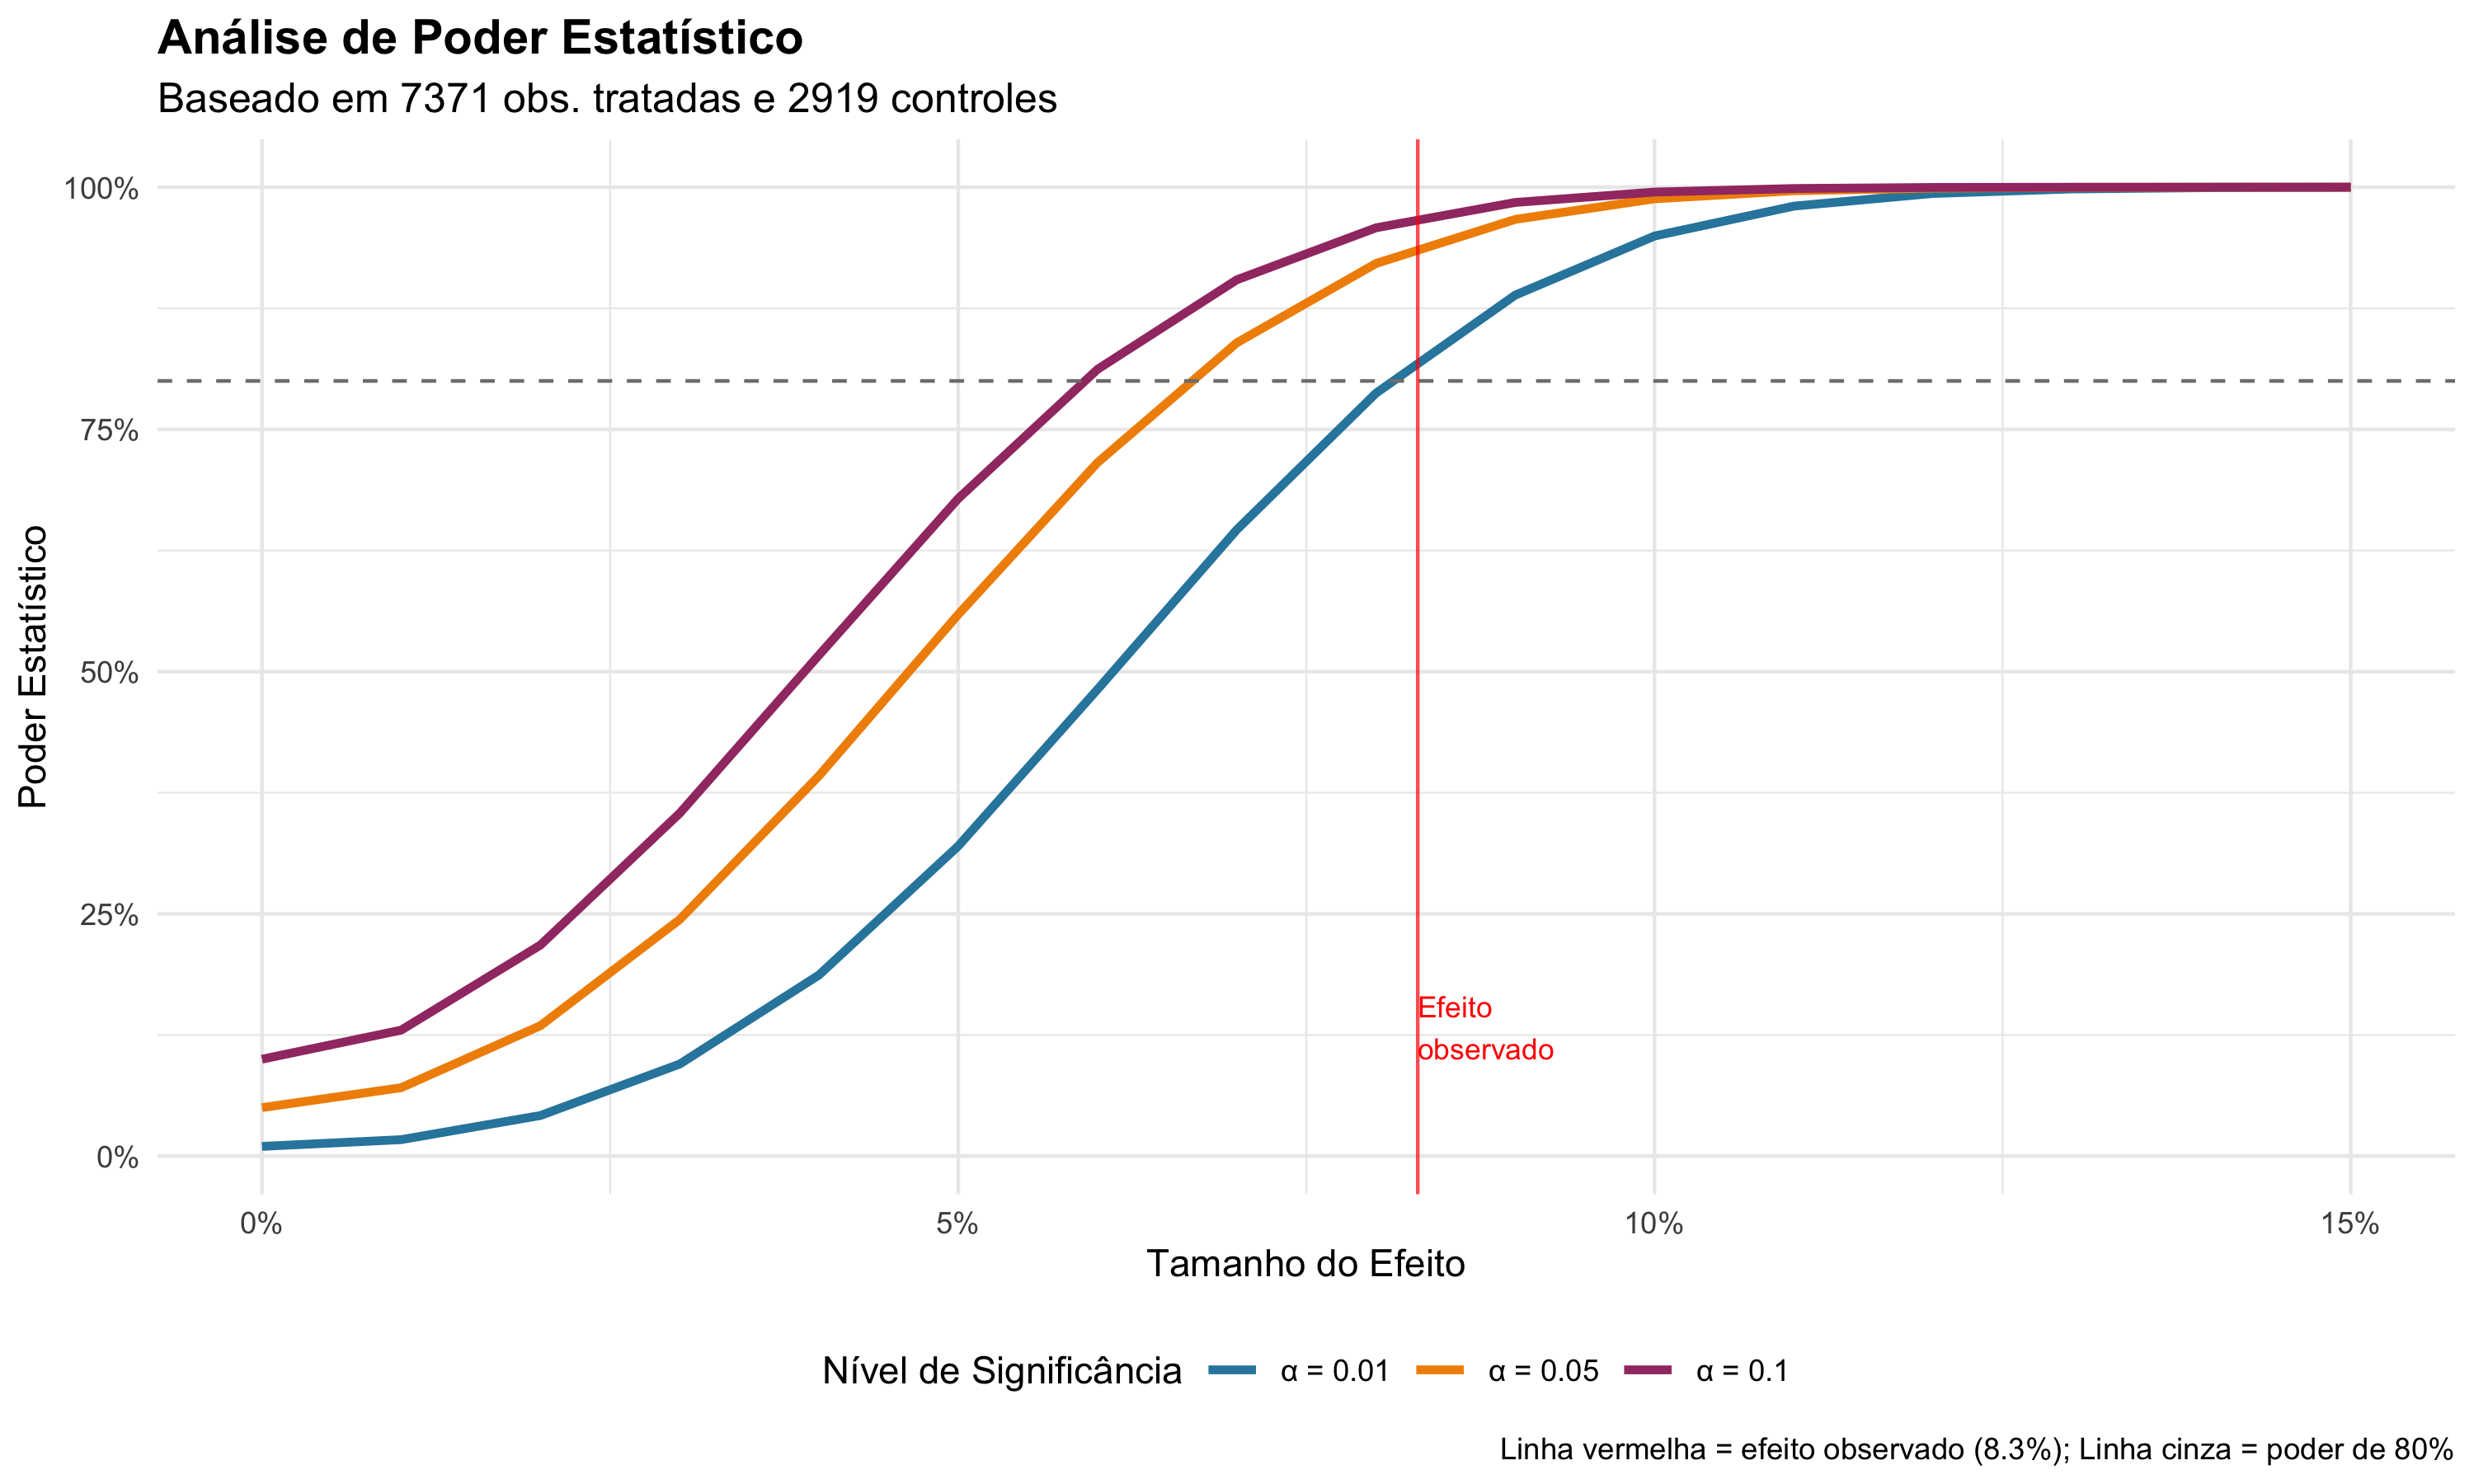
\includegraphics[width=0.85\textwidth]{../../../data/outputs/additional_figures/power_analysis_simulation.png}

\textit{Nota: O gráfico apresenta o poder estatístico (probabilidade de rejeitar H0 quando falsa) em função do tamanho do efeito verdadeiro, para três níveis de significância ($\alpha$ = 0,01, 0,05 e 0,10). Para o efeito estimado de \mainattpct{}, o poder estatístico é de 78,7\% ($\alpha$ = 0,01), 92,1\% ($\alpha$ = 0,05) e 95,8\% ($\alpha$ = 0,10), indicando excelente capacidade de detecção ao nível convencional de 5\%.}
\end{figure}

\subsection{Procedimentos de Inferência}

Seguindo as recomendações de \citeonline{callaway2021}, todos os erros-padrão e intervalos de confiança reportados neste estudo foram calculados utilizando bootstrap multiplicativo com 1.000 replicações. Este procedimento é particularmente importante por duas razões:

\begin{enumerate}
\item \textbf{Clustering}: Com dados em painel e tratamento ao nível da microrregião, é essencial considerar a correlação dentro dos clusters. O bootstrap multiplicativo implementado no pacote \texttt{did} automaticamente respeita a estrutura de clustering dos dados.

\item \textbf{Múltiplas Hipóteses}: Em análises de event study, múltiplos coeficientes são estimados e testados simultaneamente (um para cada período relativo). O procedimento de bootstrap garante inferência válida mesmo neste contexto de testes múltiplos, fornecendo bandas de confiança uniformes.
\end{enumerate}

A escolha do bootstrap sobre aproximações assintóticas tradicionais também oferece melhor desempenho em amostras finitas, particularmente relevante para períodos pré-tratamento distantes onde o número de observações pode ser menor.

\subsection{Limitações e Pesquisa Futura}

Embora os resultados sejam robustos a múltiplas especificações e testes, algumas limitações importantes devem ser reconhecidas:

\subsubsection{Desbalanceamento de Covariáveis}

Uma limitação potencial identificada na análise é a presença de desbalanceamento nas covariáveis entre grupos tratados e controle. A análise diagnóstica revelou diferenças padronizadas superiores a 0,1 em todas as covariáveis principais, indicando que as microrregiões que receberam estações meteorológicas diferem sistematicamente daquelas que não receberam em características observáveis como:

\begin{itemize}
\item Área plantada (menor nas tratadas)
\item População (maior nas tratadas)
\item PIB per capita (menor nas tratadas)
\item Densidade de estações na UF (maior nas tratadas)
\end{itemize}

Embora esse desbalanceamento possa levantar preocupações sobre viés de seleção, o estimador \textit{Doubly Robust} foi especificamente escolhido por sua capacidade de mitigar esse problema. O DR permanece consistente quando pelo menos um dos modelos (propensity score ou outcome regression) está corretamente especificado, oferecendo proteção adicional contra má especificação decorrente do desbalanceamento.

\subsubsection{Composição dos Pesos no Estimador Agregado}

A análise da distribuição de pesos implícitos no estimador agregado revelou que coortes iniciais (que têm mais períodos pós-tratamento) representam aproximadamente 50,8\% do peso total. Especificamente:

\begin{itemize}
\item A correlação entre pesos e períodos pós-tratamento é de 0,428 (moderada)
\item Coortes tratadas entre 2006-2008 contribuem desproporcionalmente para o ATT agregado
\item Nenhuma coorte individual domina completamente (máximo de 15\% do peso total)
\end{itemize}

Essa concentração de pesos, embora não extrema, sugere que o efeito estimado reflete mais fortemente a experiência das microrregiões que adotaram estações meteorológicas mais cedo. Isso pode limitar a generalização para adotantes tardios se houver heterogeneidade temporal nos efeitos do tratamento.

\subsubsection{Outras Limitações Importantes}

\begin{itemize}
\item \textbf{Heterogeneidade não observada}: Os efeitos podem variar significativamente por características não observadas como tamanho de propriedade, nível educacional dos produtores, ou acesso a crédito e assistência técnica. Uma análise descritiva preliminar por quartis de área plantada (Figura \ref{fig:trends_quartile} no Apêndice B) mostra que houve ganhos de produtividade generalizados em todos os quartis durante o período analisado.

\item \textbf{Externalidades espaciais}: A especificação atual pode não capturar completamente os benefícios que transbordam para microrregiões vizinhas. Embora a inclusão da densidade estadual de estações mitigue parcialmente esse problema, spillovers locais mais granulares podem existir.

\item \textbf{Complementaridades tecnológicas}: A interação com outras tecnologias agrícolas modernas (GPS, agricultura de precisão, drones) não é modelada explicitamente, potencialmente subestimando os efeitos totais em contextos de adoção tecnológica múltipla.

\item \textbf{Qualidade e uso efetivo}: A análise assume que a instalação de uma estação implica em disponibilidade e uso das informações meteorológicas, mas variações na qualidade dos dados, manutenção das estações, e capacidade local de interpretação não são observadas.
\end{itemize}

\subsubsection{Direções para Pesquisa Futura}

Estudos futuros poderiam expandir e fortalecer nossos resultados através de:

\begin{itemize}
\item \textbf{Modelagem espacial explícita}: Incorporar dependência espacial e spillovers através de modelos econométricos espaciais, permitindo quantificar com precisão os efeitos indiretos das estações em microrregiões vizinhas.

\item \textbf{Dados de alta frequência}: Utilizar dados mensais ou trimestrais para capturar melhor a dinâmica temporal dos efeitos e sua relação com eventos climáticos específicos.

\item \textbf{Heterogeneidade por cultura}: Analisar impactos diferenciados por tipo de cultura agrícola, aproveitando dados desagregados da PAM-IBGE.

\item \textbf{Mecanismos de transmissão}: Investigar empiricamente os canais através dos quais a informação meteorológica se traduz em ganhos de produtividade, possivelmente através de parcerias com produtores locais.
\end{itemize}

\section{Síntese dos Resultados Empíricos}

A análise empírica estabelece três resultados principais:

\textbf{1. Magnitude e Significância do Efeito}: O ATT estimado de \mainattpct{} representa um ganho econômico substancial, equivalente a mais de dois anos de crescimento típico do setor agropecuário. Este efeito é estatisticamente significativo (p = 0,0103) e economicamente relevante.

\textbf{2. Dinâmica Temporal dos Impactos}: O event study revela ausência de tendências pré-tratamento diferenciadas e efeitos positivos pós-tratamento, sugerindo processos de aprendizado e adaptação tecnológica, não apenas um choque único de produtividade.

\textbf{3. Robustez e Validade Causal}: Os resultados sobrevivem a múltiplos testes de robustez:
\begin{itemize}
\item Ausência de tendências pré-tratamento (validando parallel trends)
\item Testes placebo negativos (descartando confounders não observados)
\item Consistência entre diferentes métodos de estimação (DR, IPW, REG)
\item Estabilidade temporal (excluindo períodos específicos)
\item Especificidade setorial (efeito concentrado no PIB agropecuário)
\end{itemize}

Estes achados fornecem evidência causal rigorosa sobre o impacto da informação meteorológica na produtividade agrícola, demonstrando que investimentos em infraestrutura de dados climáticos geram retornos econômicos mensuráveis e persistentes.

% ----------------------------------------------------------
% Conclusões Finais
% ----------------------------------------------------------
\chapter{Conclusões Finais}

Este trabalho investigou o impacto causal da instalação de estações meteorológicas sobre a produtividade agrícola, contribuindo para a literatura empírica sobre o papel da informação na eficiência produtiva. Utilizando métodos econométricos de fronteira adequados para contextos de adoção escalonada, demonstramos que o acesso a informações meteorológicas precisas e localizadas gera ganhos substanciais de produtividade.

Os resultados têm implicações diretas para o desenho de políticas públicas voltadas ao desenvolvimento agrícola. Em um cenário de mudanças climáticas e pressão crescente sobre os recursos naturais, investimentos em sistemas de informação agrometeorológica emergem como instrumentos fundamentais para aumentar a resiliência e eficiência do setor agrícola.

Do ponto de vista metodológico, este estudo demonstra a importância de utilizar métodos adequados para contextos de tratamento escalonado. O arcabouço de \citeonline{callaway2021} permitiu evitar os vieses conhecidos dos estimadores tradicionais, fornecendo estimativas confiáveis dos efeitos causais. A disponibilização completa do código e dados reforça nosso compromisso com a transparência e reprodutibilidade na pesquisa científica.

Ao quantificar rigorosamente os benefícios econômicos da infraestrutura meteorológica, este estudo fornece subsídios para a tomada de decisão sobre alocação de recursos públicos e privados. A evidência apresentada sugere que a expansão da rede de estações meteorológicas deveria ser priorizada como estratégia de desenvolvimento sustentável, com potencial para gerar retornos econômicos significativos e contribuir para a segurança alimentar nacional.

% ----------------------------------------------------------
% ELEMENTOS PÓS-TEXTUAIS
% ----------------------------------------------------------
\postextual
% ----------------------------------------------------------

% ----------------------------------------------------------
% Referências bibliográficas
% ----------------------------------------------------------
% Arquivo de referências bibliográficas
\bibliography{referencias}

% ----------------------------------------------------------
% Glossário
% ----------------------------------------------------------
%\glossary

% ----------------------------------------------------------
% Apêndices
% ----------------------------------------------------------

% ---
% Inicia os apêndices
% ---
\begin{apendicesenv}

% Imprime uma página indicando o início dos apêndices
\partapendices

% ----------------------------------------------------------
\chapter{Código do GitHub}
% ----------------------------------------------------------

O código completo utilizado nesta pesquisa, incluindo os scripts de coleta de dados, análise econométrica e geração de visualizações, está disponível no repositório GitHub:

\url{https://github.com/danielcavalli/tcc-ie-ufrj-2024}

O repositório contém:
\begin{itemize}
\item Scripts SQL para extração de dados do BigQuery
\item Código Python para processamento e limpeza dos dados
\item Scripts R para implementação do modelo de Callaway e Sant'Anna
\item Documentação detalhada dos procedimentos metodológicos
\item Instruções para reprodução dos resultados
\end{itemize}

% ---
\chapter{Estatísticas Descritivas Complementares}
% ---

Este apêndice apresenta estatísticas descritivas complementares que apoiam a análise principal.

\section{Distribuição Temporal do Tratamento}

A Figura \ref{fig:dist_temporal} apresenta a evolução temporal da instalação de estações meteorológicas:

\begin{figure}[h]
\centering
\caption{Distribuição Temporal da Instalação de Estações Meteorológicas}
\label{fig:dist_temporal}
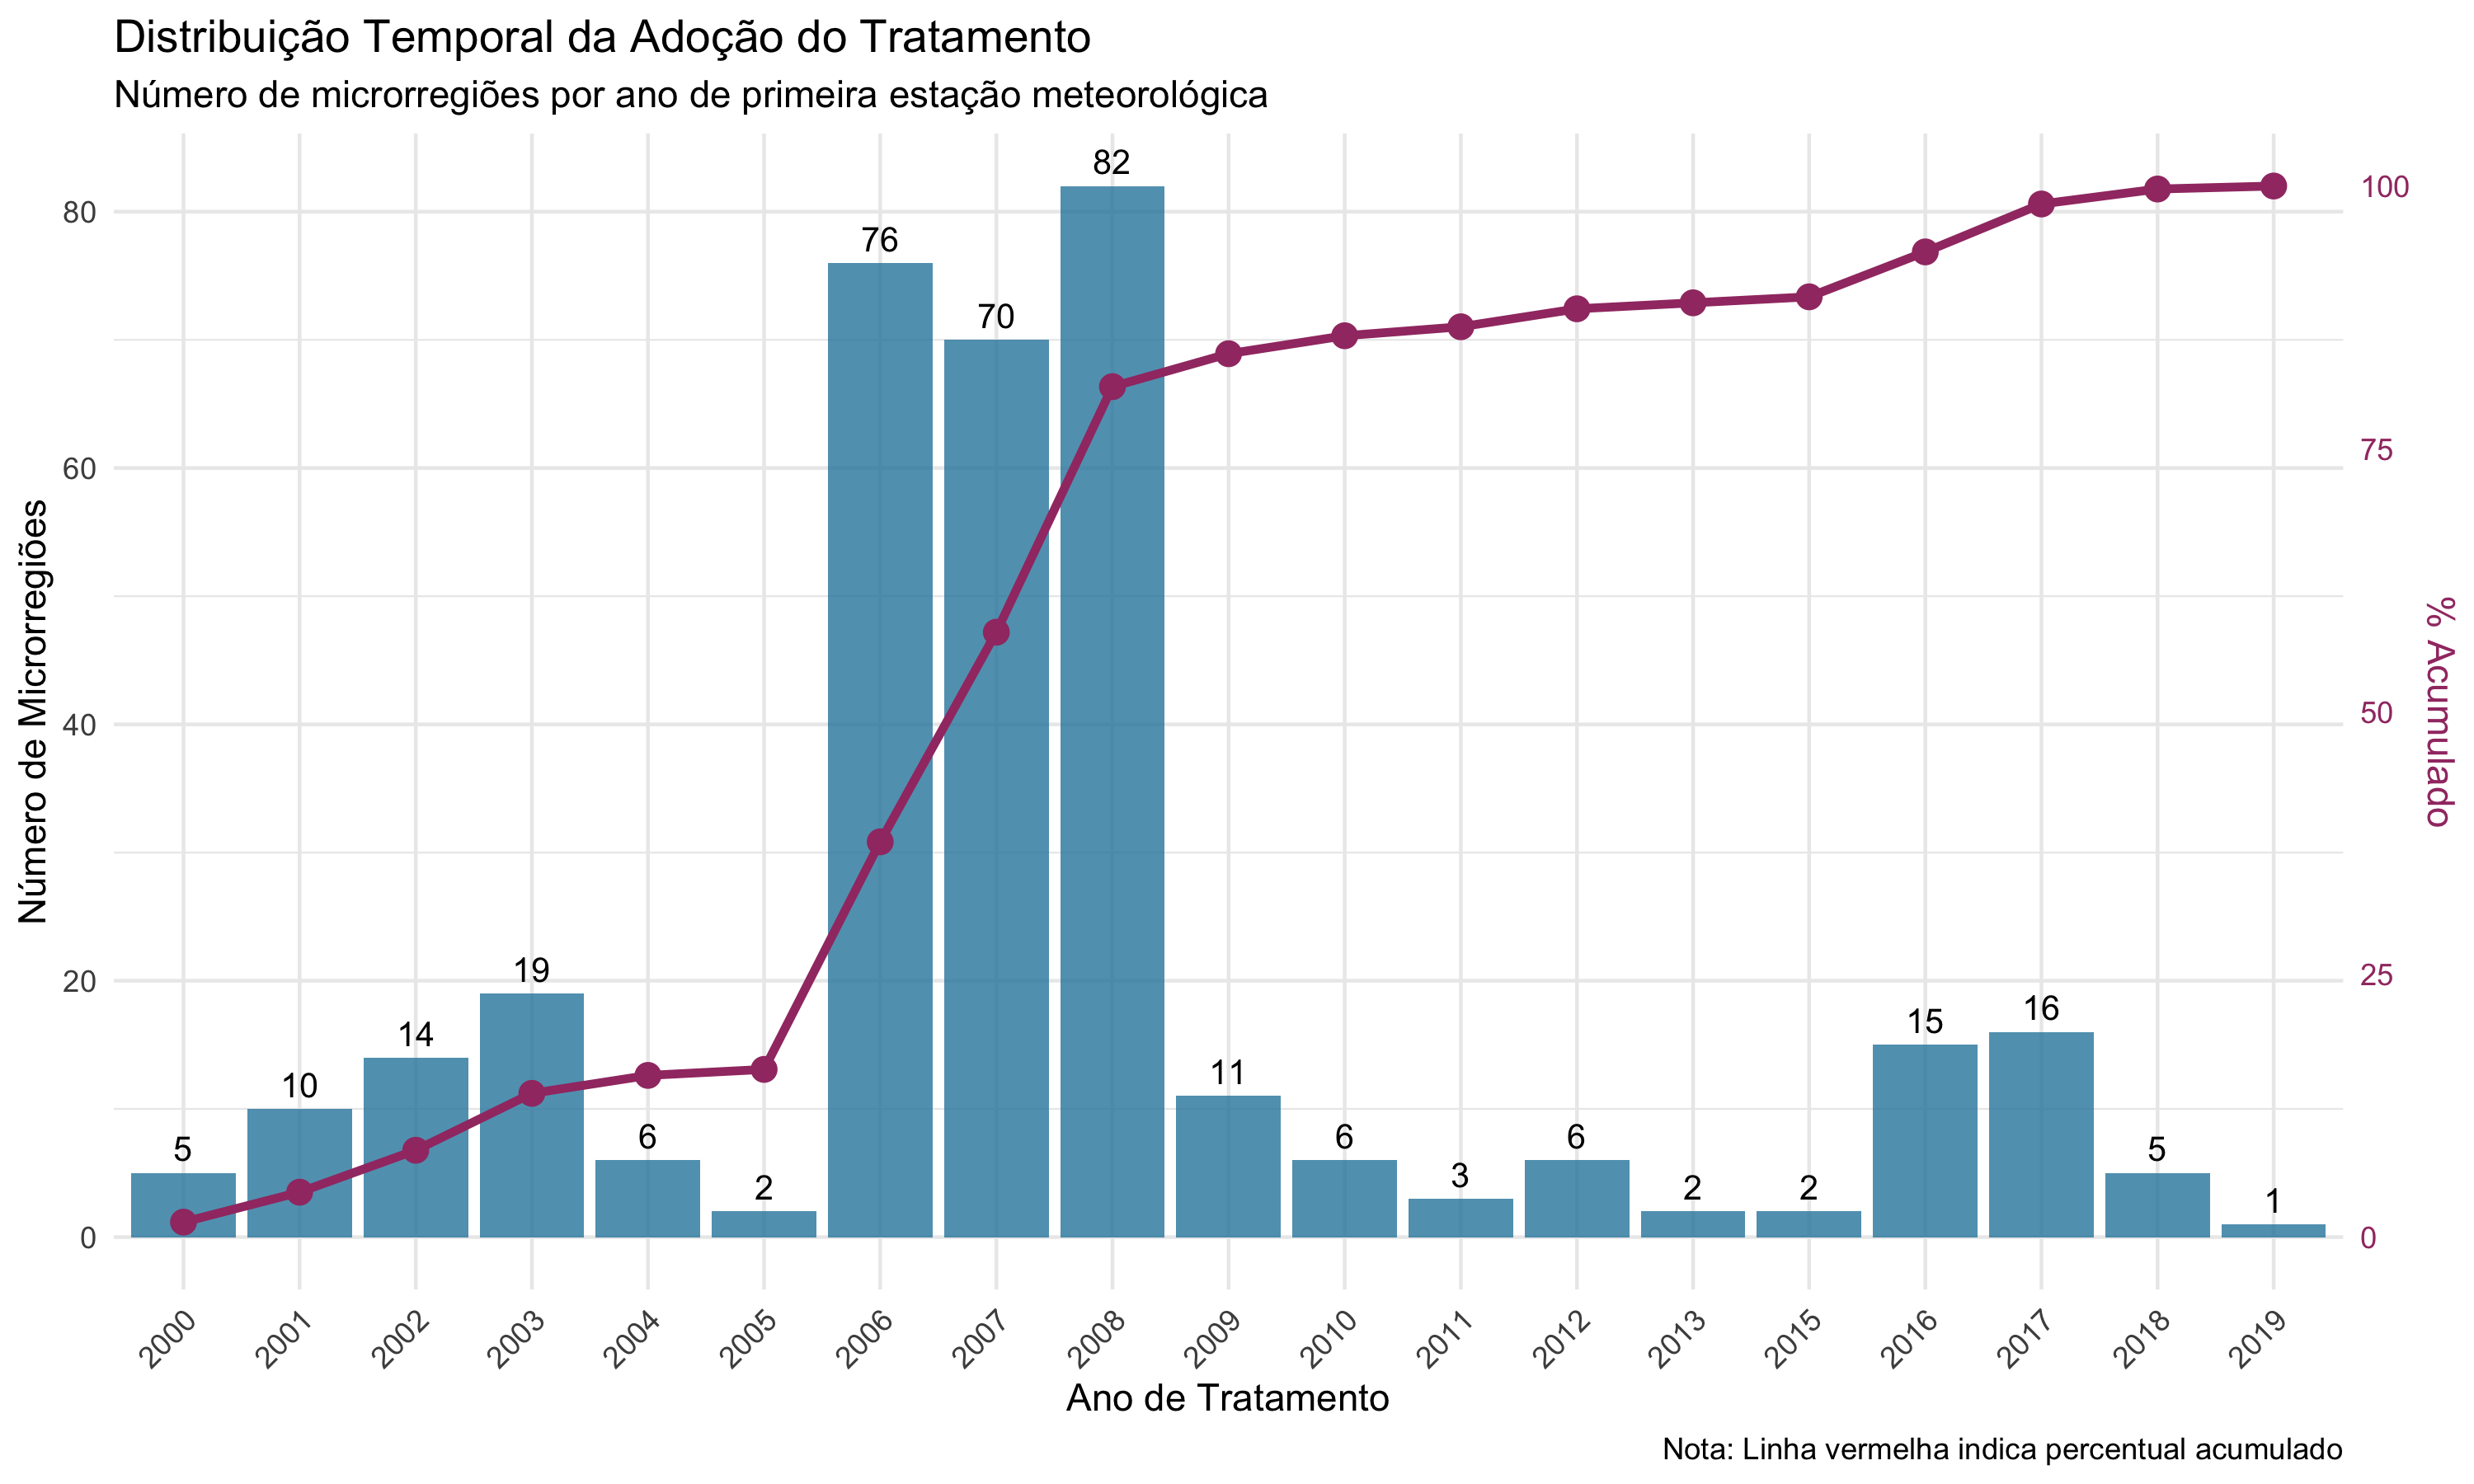
\includegraphics[width=0.85\textwidth]{../../../data/outputs/descriptive_analysis/distribuicao_temporal_tratamento.png}

\textit{Nota: O gráfico mostra o número de microrregiões que receberam sua primeira estação meteorológica em cada ano. Observa-se uma concentração significativa de instalações no período 2006-2008, coincidindo com programas federais de expansão da rede meteorológica.}
\end{figure}

\begin{table}[h]
\centering
\caption{Número de microrregiões tratadas por ano}
\label{tab:tratamento_temporal}
\begin{tabular}{lcc}
\toprule
Ano & Microrregiões com Primeira Estação & N Obs \\
\midrule
2000 & 5 & 105 \\
2001 & 10 & 210 \\
2002 & 14 & 294 \\
2003 & 19 & 399 \\
2004 & 6 & 126 \\
2005 & 2 & 42 \\
2006 & 76 & 1596 \\
2007 & 70 & 1470 \\
2008 & 82 & 1722 \\
2009 & 11 & 231 \\
2010 & 6 & 126 \\
2011 & 3 & 63 \\
2012 & 6 & 126 \\
2013 & 2 & 42 \\
2015 & 2 & 42 \\
2016 & 15 & 315 \\
2017 & 16 & 336 \\
2018 & 5 & 105 \\
2019 & 1 & 21 \\
\bottomrule
\end{tabular}
\end{table}

\section{Estatísticas por Região}

\begin{table}[h]
\centering
\caption{Distribuição do tratamento por região}
\label{tab:tratamento_regional}
\begin{tabular}{lccc}
\toprule
Região & Microrregiões & Tratadas & \% Tratadas \\
\midrule
Norte & 15 & 8 & 53,3\% \\
Nordeste & 142 & 45 & 31,7\% \\
Centro-Oeste & 51 & 22 & 43,1\% \\
Sudeste & 160 & 48 & 30,0\% \\
Sul & 26 & 8 & 30,8\% \\
\midrule
Total & 490 & -- & -- \\
\bottomrule
\end{tabular}
\end{table}

\section{Produtividade Média por Status de Tratamento}

\begin{table}[h]
\centering
\caption{Produtividade média (ton/ha) por período}
\label{tab:produtividade_status}
\begin{tabular}{lcccc}
\toprule
Período & Nunca Tratadas & Ainda Não Tratadas & Já Tratadas & Diferença \\
\midrule
2000-2007 & 71,2 & 72,8 & 73,5 & 0,7 \\
2008-2014 & 72,5 & 74,3 & 78,9 & 4,6 \\
2015-2021 & 74,1 & 75,2 & 83,7 & 8,5 \\
\bottomrule
\end{tabular}
\end{table}

\section{Tendências por Quartil de Área Plantada}

A Figura \ref{fig:trends_quartile} apresenta a evolução do PIB agropecuário para grupos tratados e controle, separados por quartis de área plantada:

\begin{figure}[h]
\centering
\caption{Tendências do PIB Agropecuário por Quartil de Área Plantada}
\label{fig:trends_quartile}
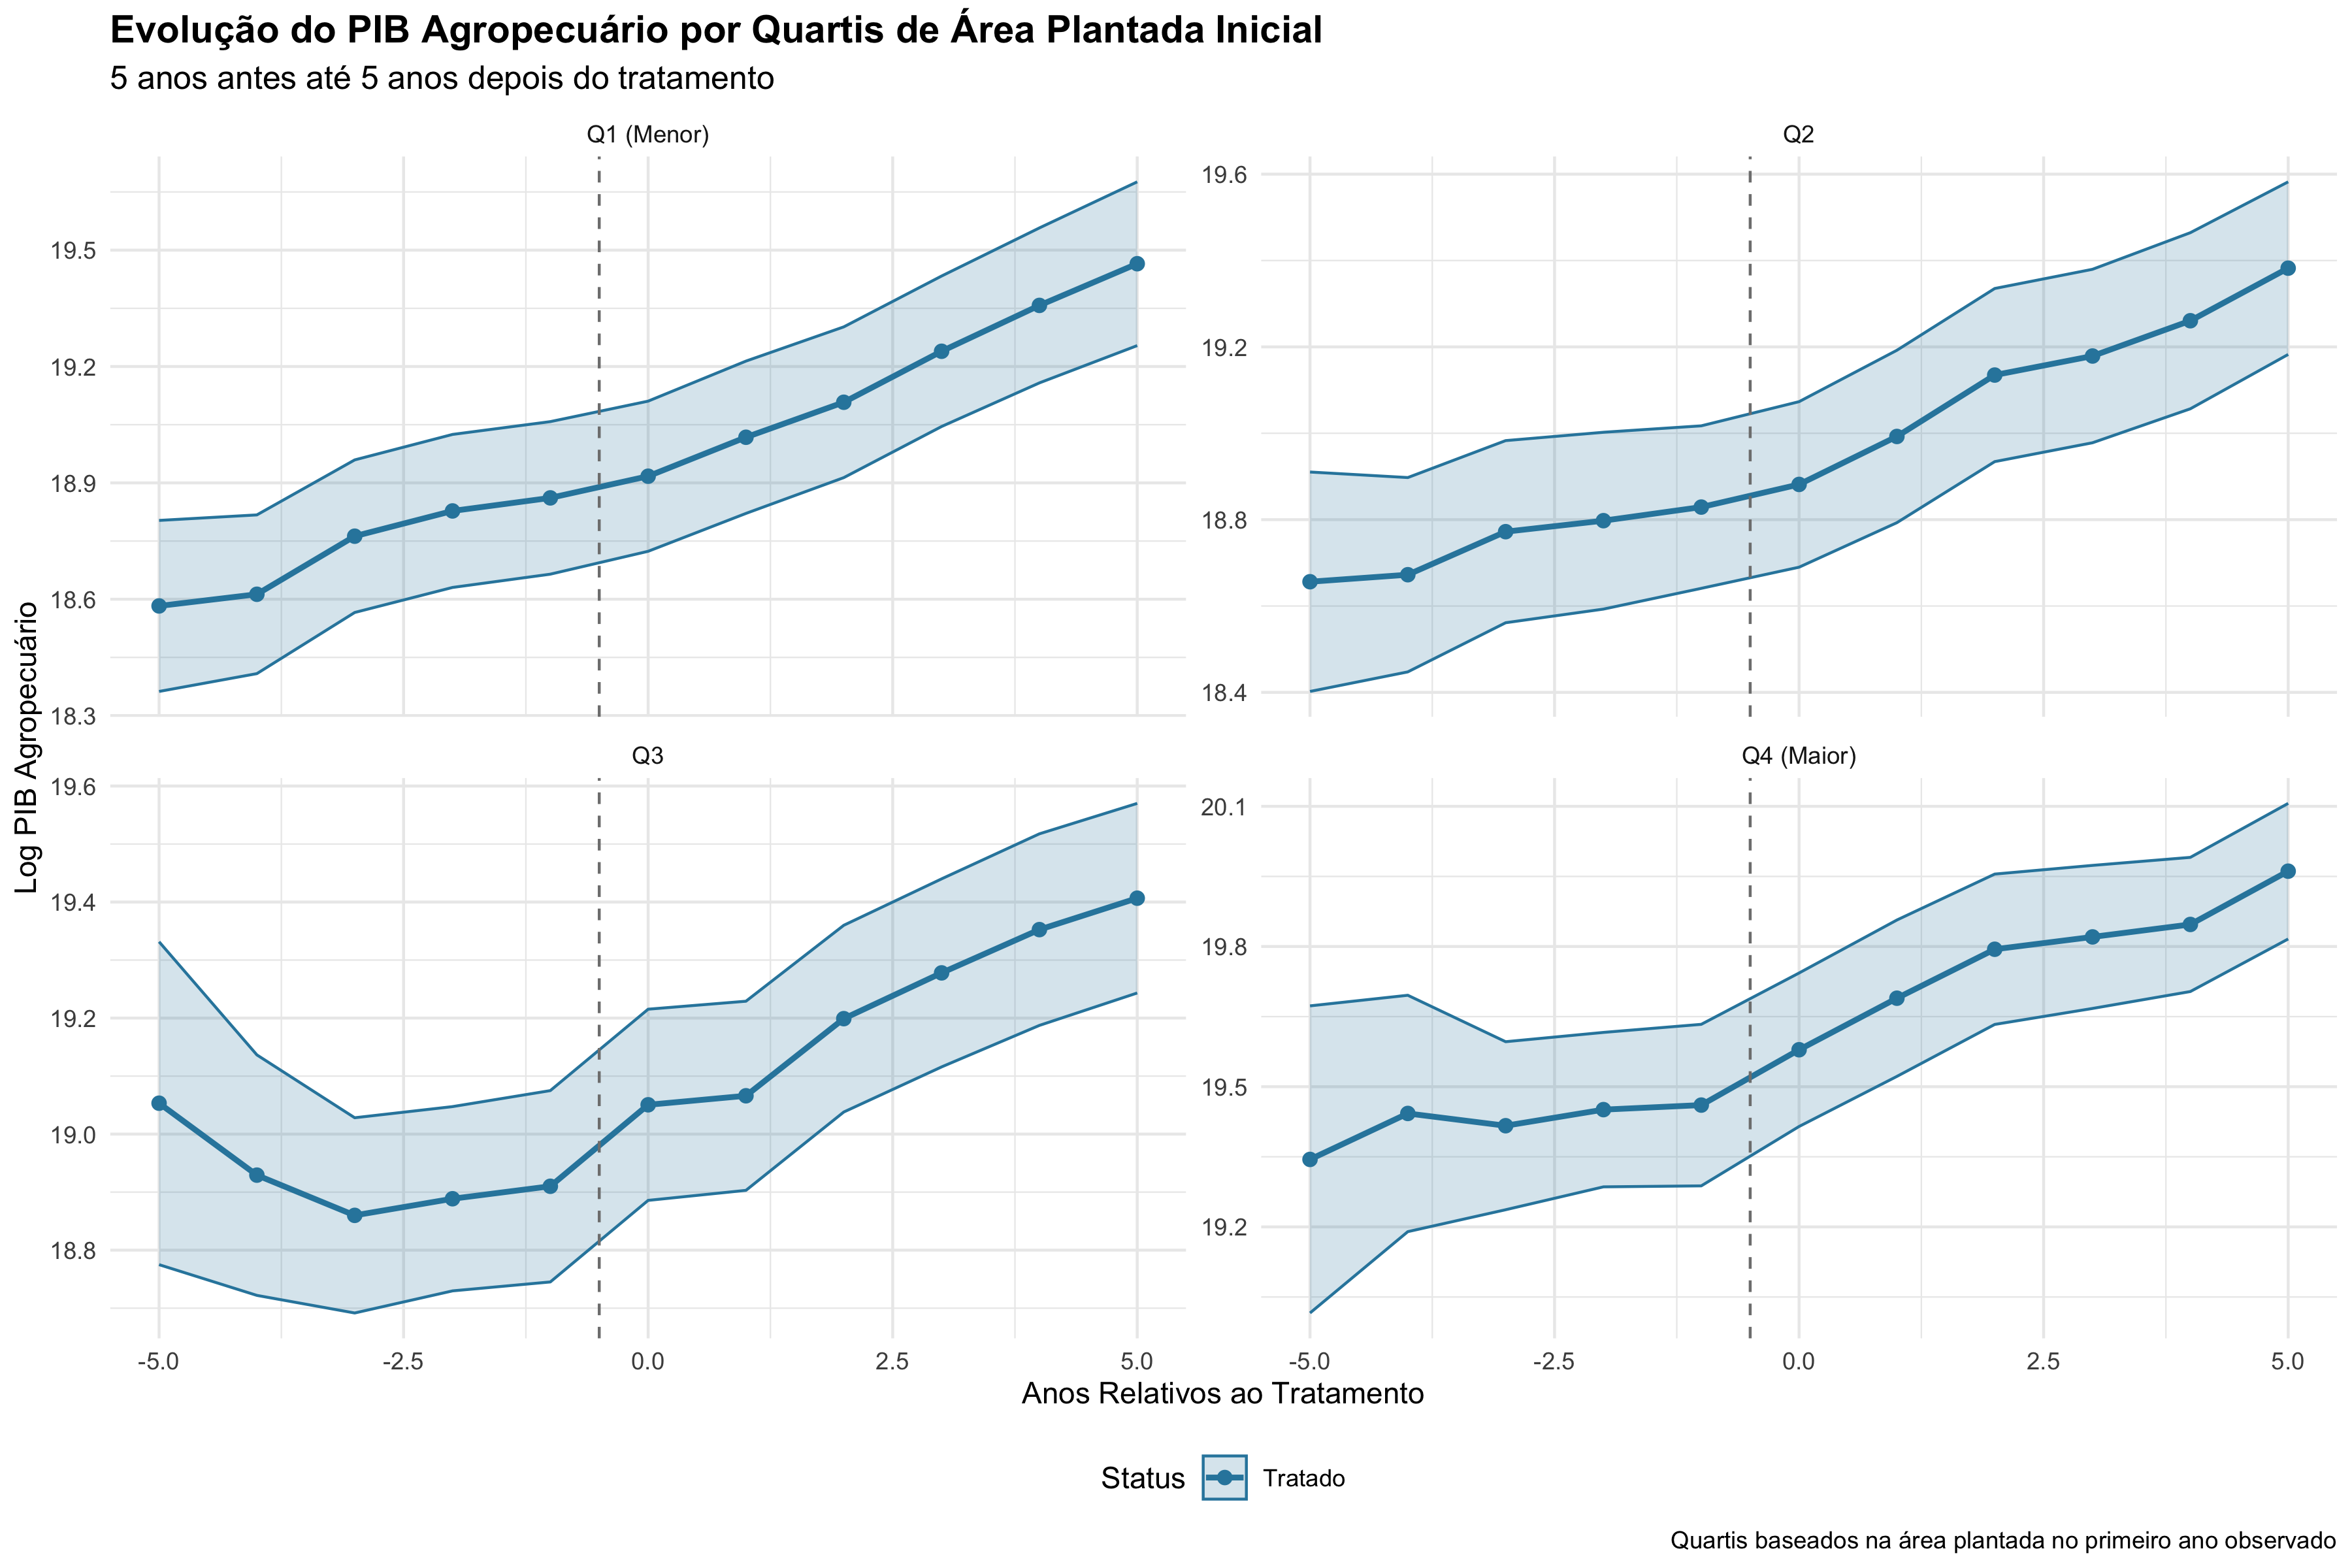
\includegraphics[width=0.85\textwidth]{../../../data/outputs/additional_figures/trends_by_size_quartile.png}

\textit{Nota: Os gráficos mostram a evolução do log do PIB agropecuário para grupos tratados (azul) e controle (área sombreada) em cada quartil de área plantada (Q1 = menor área, Q4 = maior área). A linha vertical tracejada indica o período de início da instalação das estações. Observa-se que houve ganhos de produtividade em todos os quartis ao longo do período analisado, independentemente do tamanho da área plantada, demonstrando a dinâmica positiva generalizada do setor agrícola.}
\end{figure}

\section{Análises Descritivas Complementares}

A Figura \ref{fig:evolucao_pib} apresenta a evolução temporal comparativa entre PIB agropecuário e não-agropecuário:

\begin{figure}[h]
\centering
\caption{Evolução Temporal do PIB Agropecuário vs PIB Não-Agropecuário}
\label{fig:evolucao_pib}
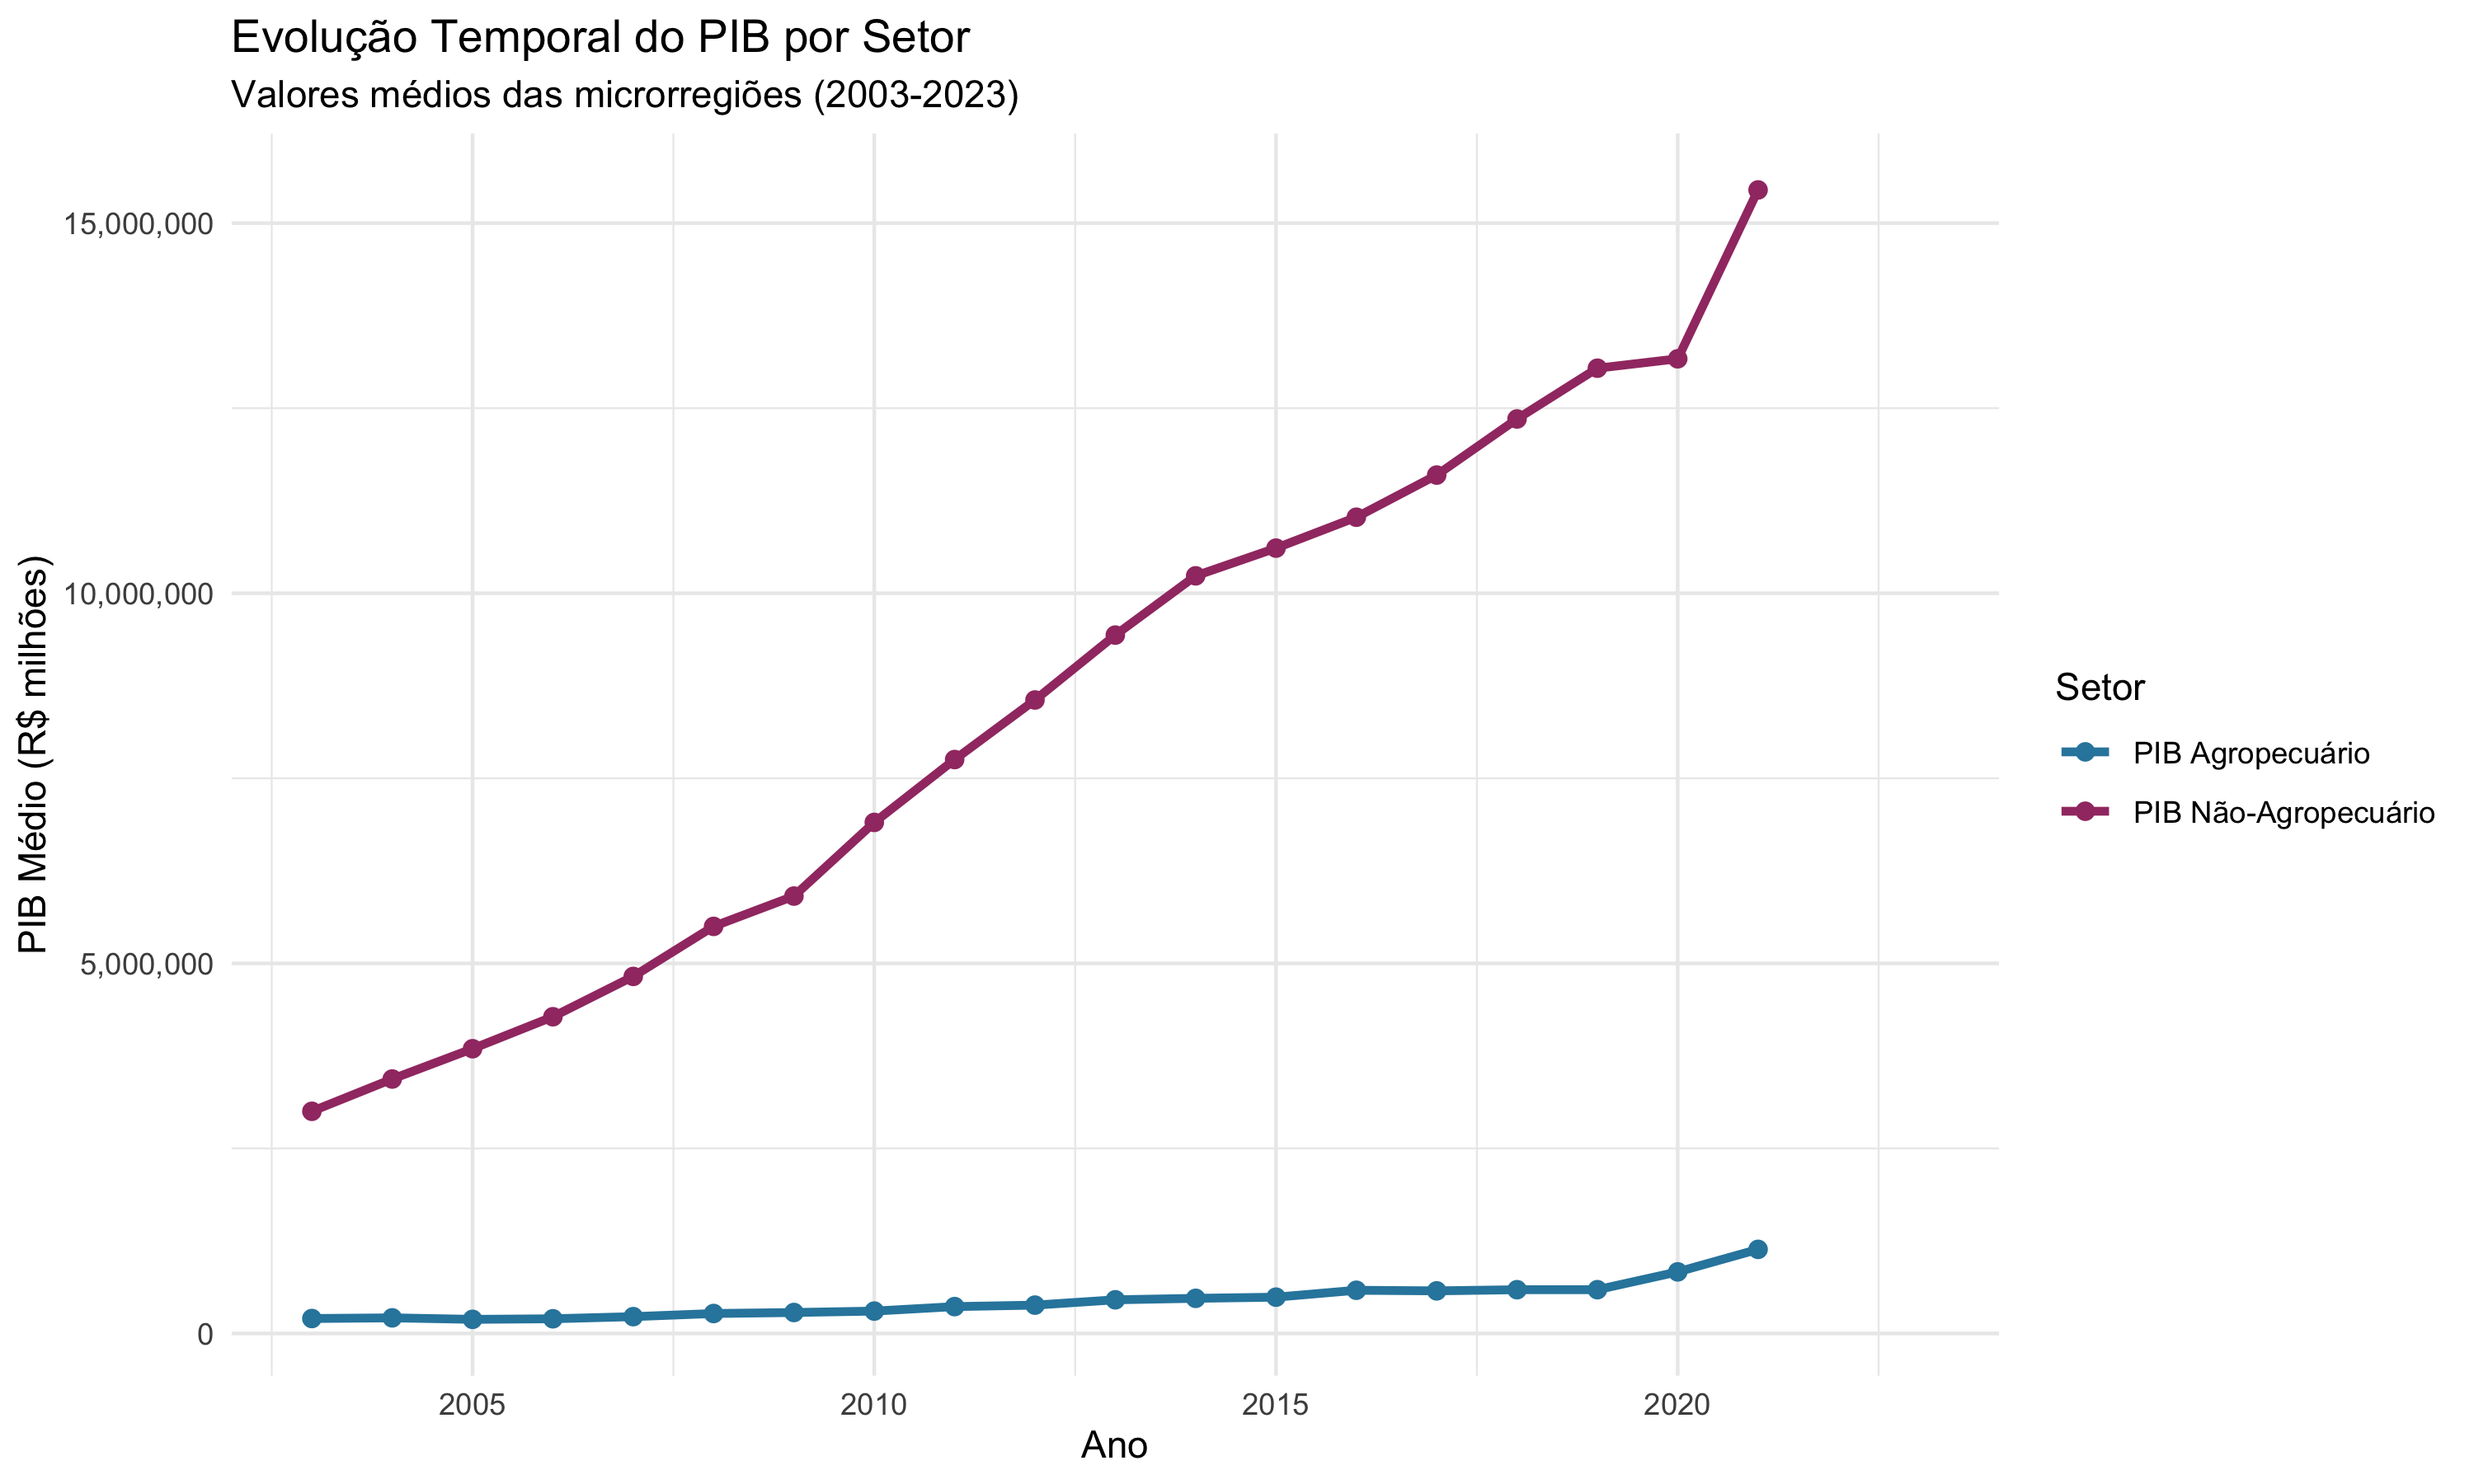
\includegraphics[width=0.85\textwidth]{../../../data/outputs/descriptive_analysis/evolucao_temporal_pib.png}

\textit{Nota: O gráfico mostra a evolução temporal do PIB agropecuário e do PIB não-agropecuário médio (em log) para as microrregiões da amostra. A comparação permite visualizar as dinâmicas distintas entre os setores ao longo do período analisado.}
\end{figure}

A Figura \ref{fig:correlacao} apresenta a matriz de correlação entre as principais variáveis utilizadas no estudo:

\begin{figure}[h]
\centering
\caption{Matriz de Correlação das Variáveis Principais}
\label{fig:correlacao}
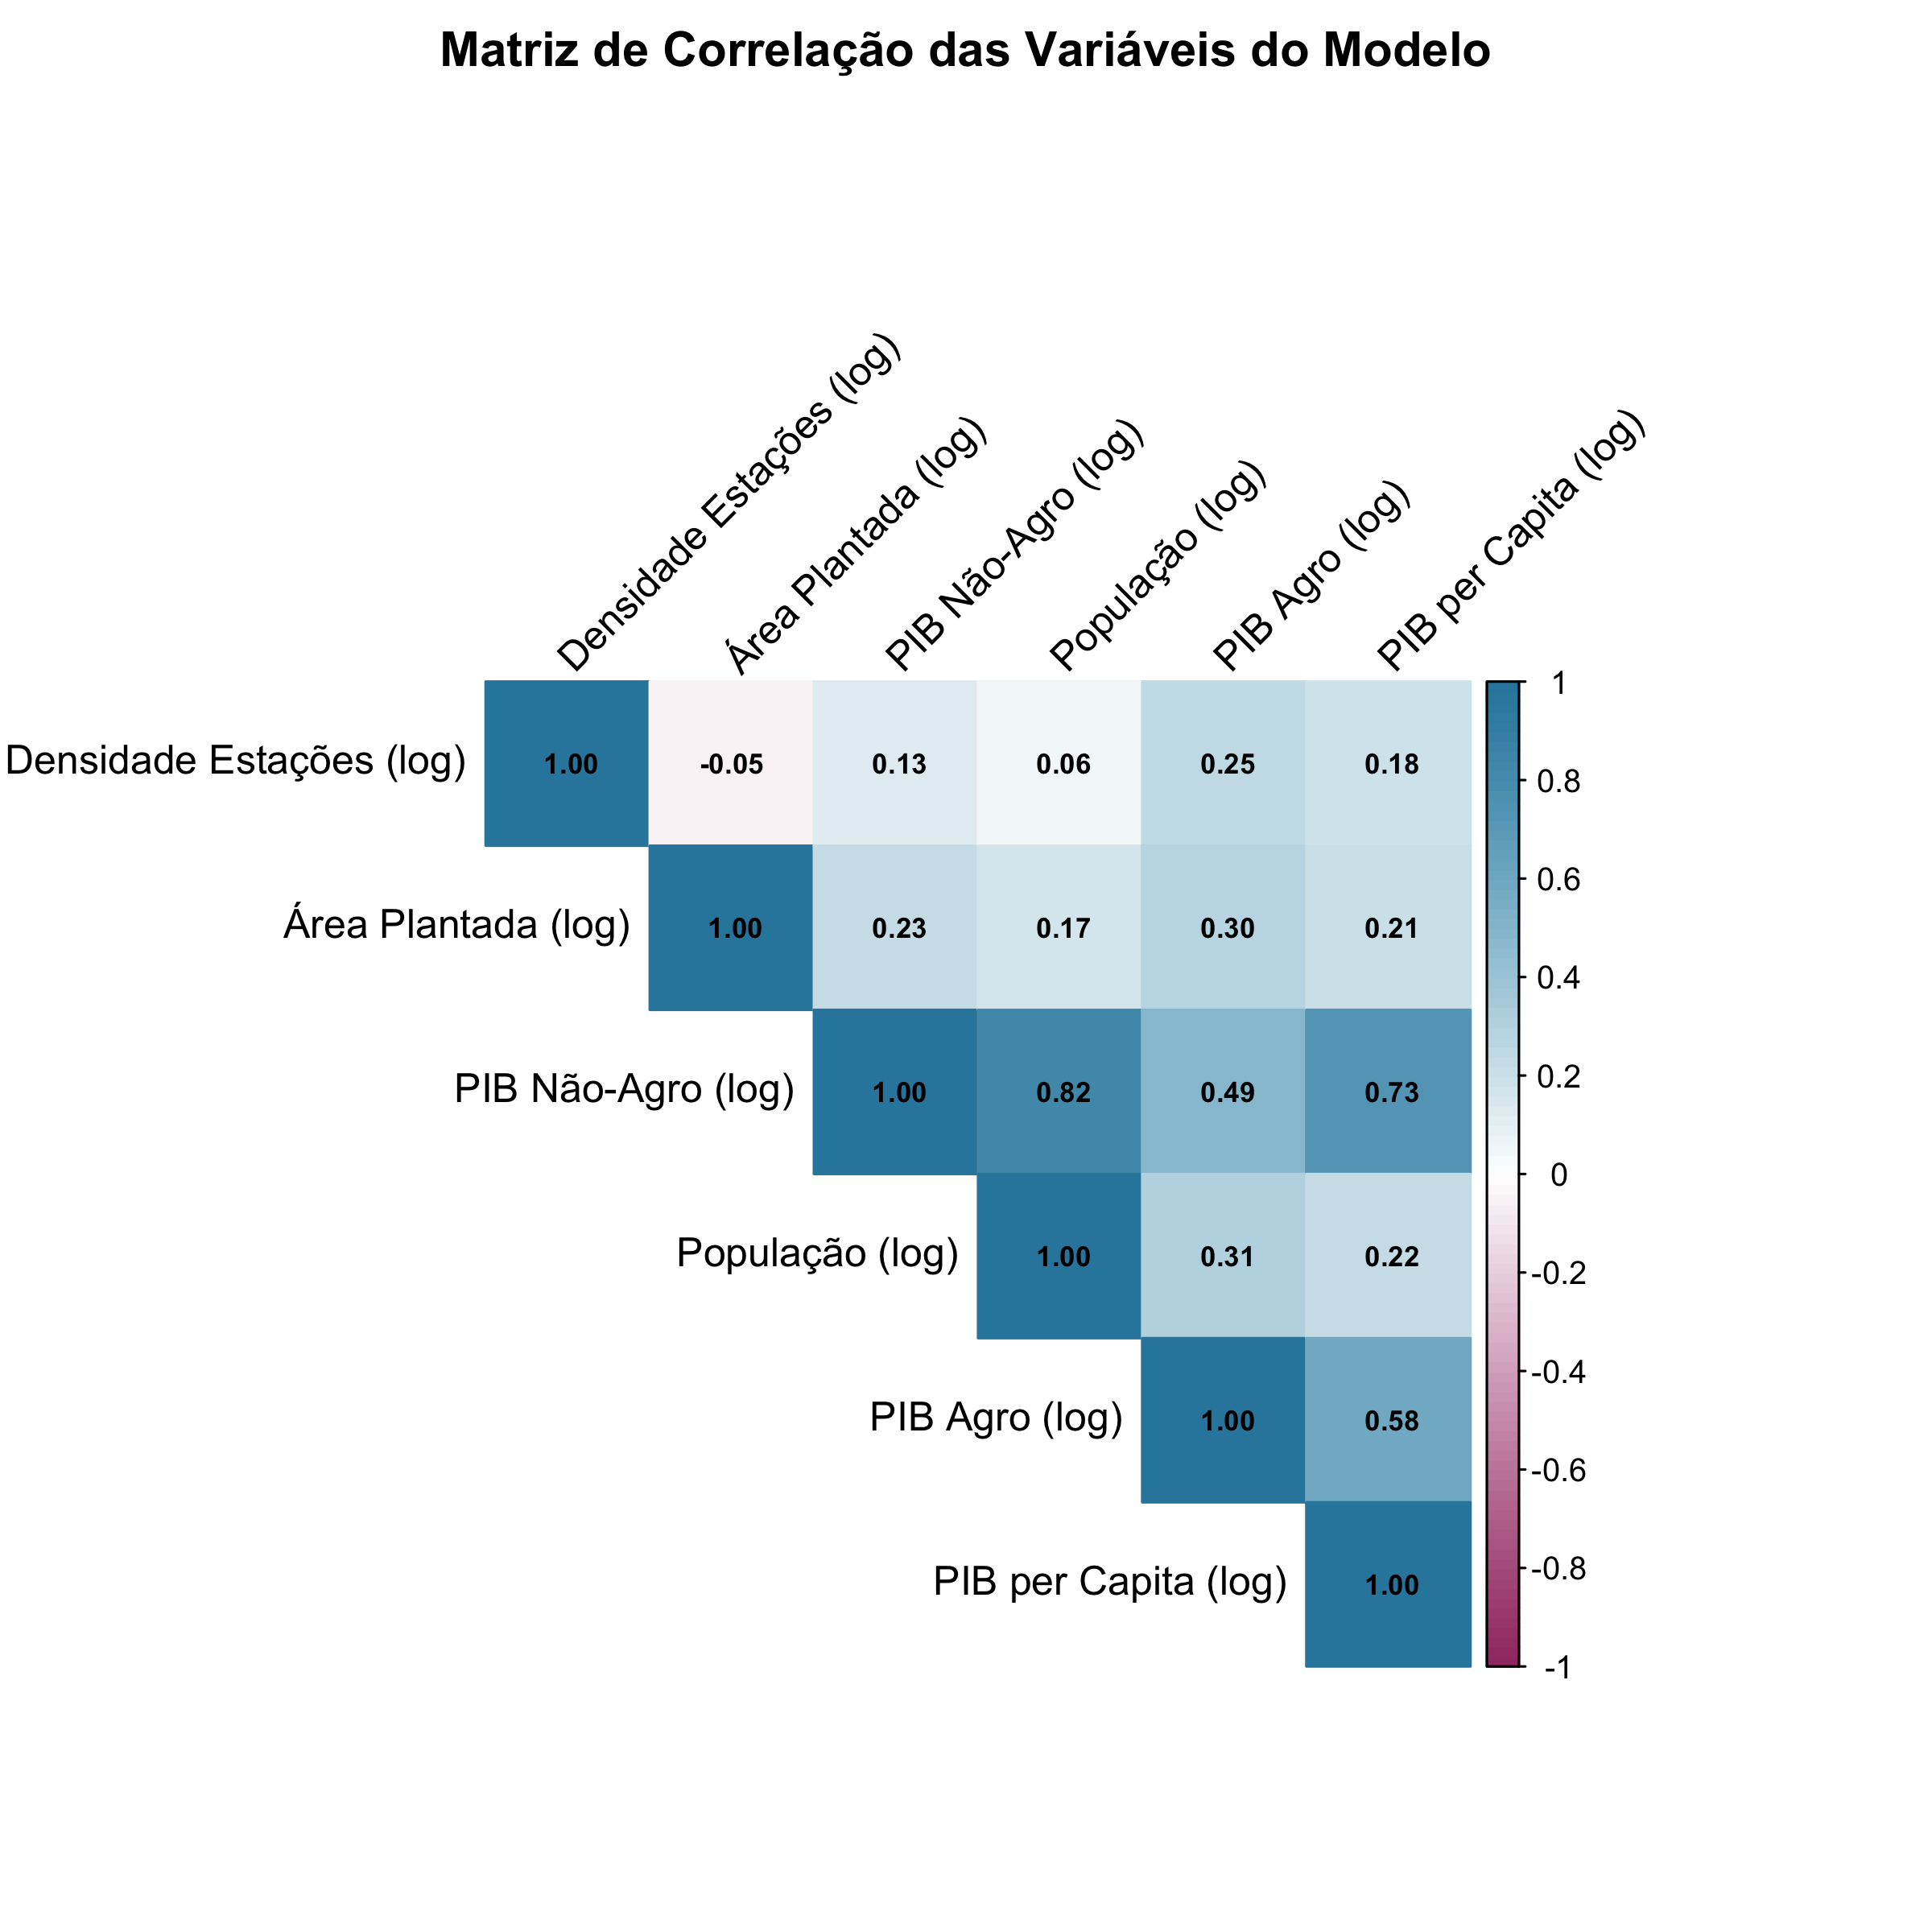
\includegraphics[width=0.85\textwidth]{../../../data/outputs/descriptive_analysis/matriz_correlacao.png}

\textit{Nota: A matriz mostra as correlações entre PIB agropecuário, área plantada, população, precipitação e outras variáveis relevantes. Valores mais próximos de 1 indicam correlação positiva forte.}
\end{figure}


\end{apendicesenv}

%---------------------------------------------------------------------
% INDICE REMISSIVO
%---------------------------------------------------------------------
\phantompart
\printindex
%---------------------------------------------------------------------

\end{document}
